\documentclass[]{project_plan}
\usepackage{graphicx, subcaption}
\usepackage{hyperref}
\usepackage{xcolor}
\usepackage{cite}
\usepackage{ upgreek, amsmath  }
\usepackage{listings, xcolor}
\usepackage{caption, wrapfig}


\definecolor{codegreen}{rgb}{0,0.6,0}
\definecolor{codegray}{rgb}{0.5,0.5,0.5}
\definecolor{codepurple}{rgb}{0.58,0,0.82}
\definecolor{backcolour}{rgb}{245,244,243}

\lstdefinestyle{mycodestyle}{
    backgroundcolor=\color{backcolour},
    commentstyle=\color{codegreen},
    keywordstyle=\color{magenta},
    numberstyle=\tiny\color{codegray},
    stringstyle=\color{codepurple},
    basicstyle=\ttfamily,
    breakatwhitespace=false,
    breaklines=true,
    captionpos=b,
    keepspaces=true,
    numbers=left,
    numbersep=5pt,
    showspaces=false,
    showstringspaces=false,
    showtabs=false,
    tabsize=2
}

\lstset{style=mycodestyle}


\newcommand{\bulletPoint}{\hspace{-3.1pt}$\bullet$ \hspace{5pt}}
\setcounter{tocdepth}{7}


%---

\def\studentname{Faeq}
\def\projecttitle{User-Centered Design}

%---

\begin{document}
\tableofcontents\pdfbookmark[0]{Table of Contents}{toc}\newpage

%---

\chapter{Lecture 1 - Introduction}

\section{Users}
What is displayed is not necessarily what is perceived

When taking into account the user, think about psychological human factors\\
“Above the neck factors”

Sometimes referred to as ‘cognitive ergonomics’ or ‘cognitive engineering’

Applications of this is applied beyond the laboratory; e.g., in industry,
schools, medicine and sports.

Human ‘error’ is normal; we know how users behave under stress so we should
design for it

\subsection{Modulatory Factors}

\begin{itemize}
  \item Individual differences - age, background, different abilities, different attitudes
  \item Stress/fatigue
  \item Organizational/societal factors
  \item Expertise
\end{itemize}

We should try to know our users;
\begin{itemize}
  \item Who are they?
  \item Talk to them
  \item Watch them
  \item Measure them
\end{itemize}

Use your imagination to establish example users - Personas

\section{Interaction Design}

Design\\
A design is a plan or specification for the construction of an object or system\\
or                                  for the implementation of an activity or process,\\
or the result of that plan or specification in the form of a prototype, product or process.

Interaction\\
Communication between a user and a system\\
• Two-way communication\\
• Several stages

Interaction design\\
Achieving goals within constraints\\
• Goals (purpose) - who is it for, why do they want it\\
• Constraints - materials, platforms, cost, safety\\
• Trade-offs - functionality/simplicity, quality/cost

Constraints\\
• Ergonomic - minimum button size\\
• Physical - high-voltage switches are big\\
• Legal and safety - high cooker controls\\
• Context and environment - easy to clean\\
• Aesthetic - must look good\\
• Economic - cost of production is always a concern

To design for interactions with computers;\\
• Understand computers - limitations, capacities, tools, platforms\\
• Understand people - psychology, sociology, human error\\
• Understand their interaction - how, when, why, etc.

\subsection{Interaction styles}

\begin{figure}[h!]
  \centering
  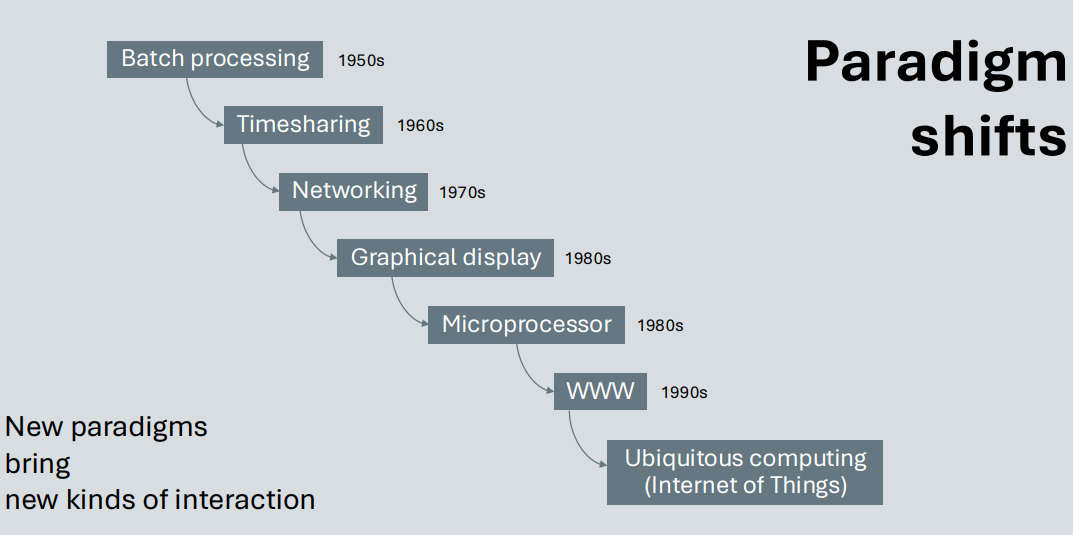
\includegraphics[width=\linewidth]{paradigm_shifts.png}
\end{figure}

• Command line interface (CLI) - Suitable for repetitive tasks - Better for expert users than novices

• Menus - Set of options displayed on the screen - Less recall, but names should be meaningful

• WIMP - Windows, Icons, Menus, Pointers - Default style for most desktops and laptops

• Point and click - Multimedia, Web browsers, hypertext - Click on icons, text links, location on map

• Natural language - Familiar to user - Speech recognition or typed

• Question/answer interfaces - Suited for novices but restricted functionality - Often used in information systems

• Form-fills - Primarily for data entry or data retrieval - Require validation/correction facilities

• Three-dimensional interfaces - VR (virtual reality) - 3D workspaces

Controllers;\\
• Menus, forms, command line and direct manipulation\\
• Touchscreens\\
• Control by speech\\
• Game console controllers\\
• Controlling with gestures\\
• Locomotion in space

\section{The Design Process}

\subsection{Donald Norman’s model}
\begin{figure}[h!]
  \centering
  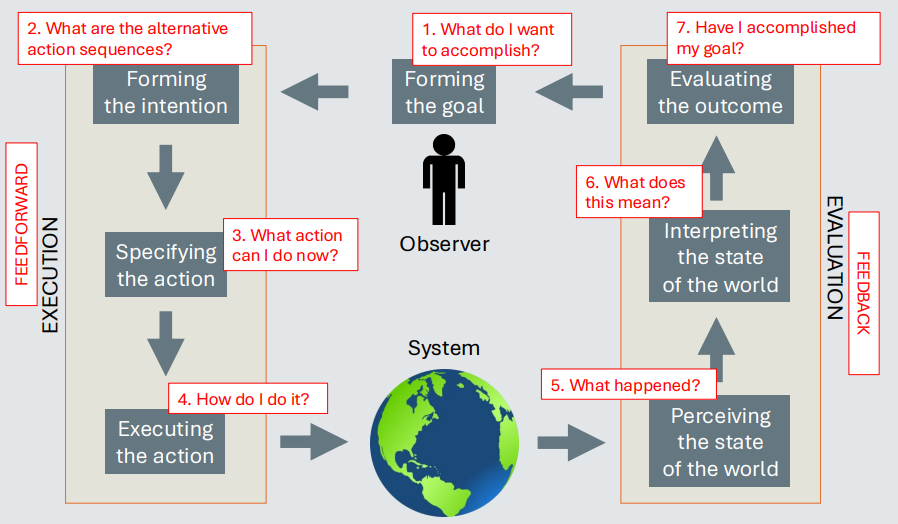
\includegraphics[width=\linewidth]{donald_norman_model.png}
\end{figure}

\newpage

\subsection{The design process}
\begin{figure}[h!]
  \centering
  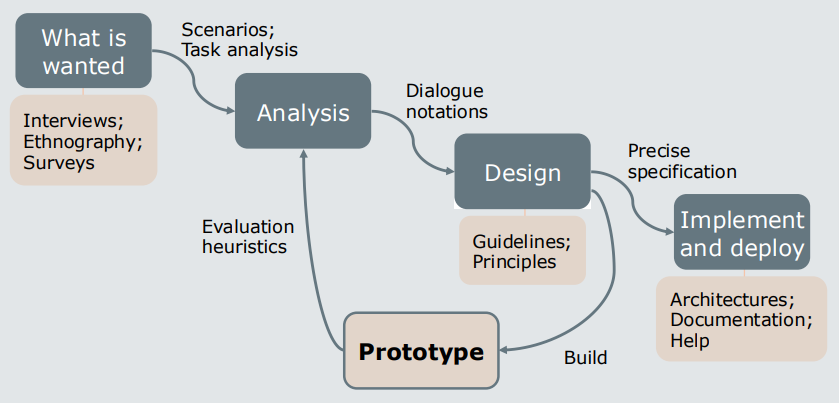
\includegraphics[width=\linewidth]{design_process.png}
\end{figure}

We are required to have ...

Trade-offs:\\
• Safety (front panel of a cooker is safer for adults, the rear panel is safer for children)\\
• Ergonomics vs physical (multifunction controls or reduced functionality)

Fluidity (physical aspects vs logical effect):\\
• Is the logical state revealed in the physical state? (on/off buttons)\\
• Do inverse actions inverse effects? (arrow buttons, twist controls)

\chapter{Workshop 1}

\section{Using Norman’s model}
The model concentrates on the user’s view of the interface\\
Some systems are harder to use than others

Users should always know;\\
• Where they are\\
• What they can do\\
• Where they are going or what will happen next\\
• Where they have been or what they’ve done

\subsection{Gulf of execution}
user’s formulation of actions $\neq$ actions allowed by the system

e.g.,
\begin{figure}[h!]
  \centering
  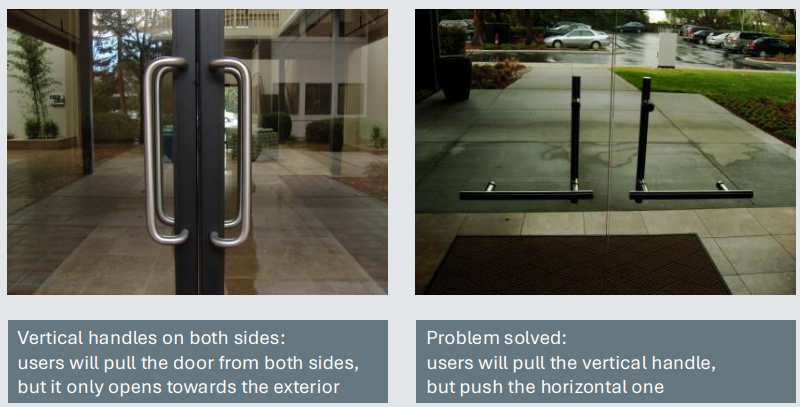
\includegraphics[width=\linewidth]{gulf_execution_example.png}
\end{figure}

\newpage

\subsection{Gulf of evaluation}
user’s expectation of changed system state $\neq$ actual presentation of the system state

e.g.,
\begin{figure}[h!]
  \centering
  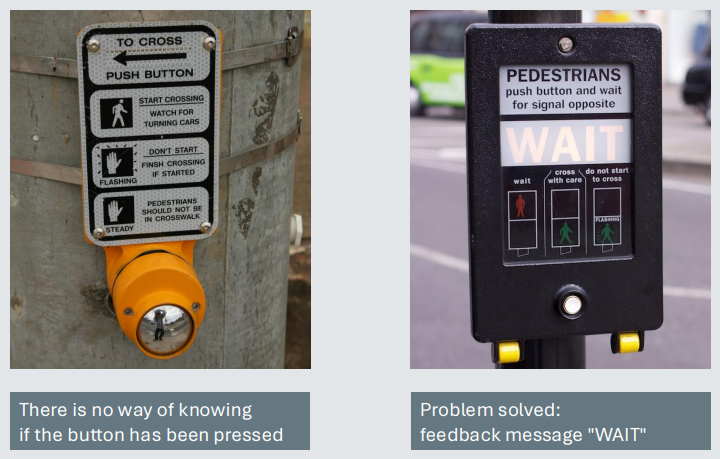
\includegraphics[width=\linewidth]{gulf_evaluation_example.png}
\end{figure}

\section{Storyboards}

Why?\\
• Maintain a user-centred mindset\\
• Identify decision making points\\
• Find potential issues\\
• Communicate ideas\\
• Express dynamics\\
- screenshots/views (appearance)\\
- scenarios (behaviour)

Storyboards include;\\
• The Main character - persona\\
• A User goal - task to complete, motivation\\
• Impediments - pain points, problems, frustrations\\
• The Location - setting, context of use\\
• The Solution - provided by the product

\newpage
e.g.,
\begin{figure}[h!]
  \centering
  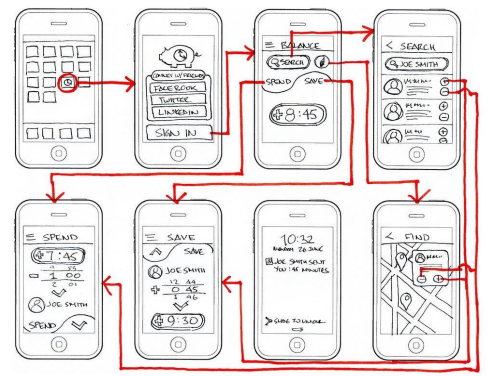
\includegraphics[width=\linewidth]{storyboard_example.png}
\end{figure}
• Represents the user journey\\
• Can be specific to one persona or general\\
• Sequences of screenshots or sketches\\
• Show the flow of transitions in response to interactions\\
• May include explicit context\\
• Normally they form a graph\\
• Each scenario is a path on the graph

\subsection{Scenarios}
A scenario is a path on the storyboard

They are stories for (user-centred) design

A step-by-step walkthrough\\
• what users see\\
• what users do\\
• what users think

A scenario is a linear path through the system

Pros\\
• life and time are linear\\
• easy to relate to\\
• concrete (errors are less likely)

\newpage

Cons\\
• no choice\\
• no branches\\
• no special conditions\\
• miss the unintended

As a result we \\
• Use several scenarios\\
• Use several methods\\
• Compile scenarios into user journeys\\
• Represent scenarios via storyboards

\section{Computers}

What is a computer?\\
• Input devices - text entry and pointing\\
• Output devices - screen (small \& large), digital paper\\
• Virtual reality - special interaction and display devices\\
• Physical interaction - sound, haptic, bio-sensing\\
• Paper - as output (print) and input (scan)\\
• Memory - RAM \& permanent media, capacity \& access\\
• Processing - speed of processing, networks

Everything is a computer;\\
At home\\
• desktop\\
• multimedia\\
• appliances\\
• central heating and cooling\\
• security system\\
With you\\
• phone/tablet\\
• camera\\
• smart card\\
• electronic car key\\
• wearables

\subsubsection{Text input}
The keyboard is the most common text input device\\
• Key press sends a character\\
• Rapid entry by experienced users\\
• Layout varies\\
• Software keyboards allow for different types of interaction (e.g. continuous input)

Other forms;\\
• Handwriting recognition\\
• Speech recognition (written or spoken)\\
• Jog dial\\
• Specialised interfaces to cope with physical disabilities\\
(controlled by different parts of the body)

\subsubsection{Pointing devices}
The mouse;\\
Handheld pointing device\\
• very common\\
• easy to use\\
• accurate and fast\\
Main characteristics\\
• planar movement\\
• buttons\\
• detects relative movement

Touchpads and touchscreens;
\begin{itemize}
  \item Stroke to move pointer
  \item Recognises gestures (multitouch) and pressure
  \item Good acceleration settings are important \begin{itemize}
          \item fast stroke \begin{itemize}
                  \item lots of pixels per inch moved
                  \item initial movement to the target
                \end{itemize}
          \item slow stroke \begin{itemize}
                  \item less pixels per inch
                  \item ideal for accurate positioning
                \end{itemize}
        \end{itemize}
\end{itemize}

Joysticks;\\
• indirect: pressure of stick corresponds to the velocity of movement\\
• buttons for selection\\
• often used for computer games, aircraft controls and 3D navigation

Pointing stick;\\
• for laptop computers and mobile phones\\
• miniature joystick in the middle of the keyboard

\subsubsection{Displays}
• LCD computer displays\\
• Large displays – meetings, lectures, etc.\\
• Situated displays – public places (display only)\\
• Interactive displays – touchscreens, boards\\
• Digital paper\\
• 3D displays – stereoscopic view, head-mounted displays (HMD)\\
• Braille displays

Dedicated displays;\\
• Analogue representations\\
• (dials, gauges, lights, etc.)\\
• Digital displays\\
• Head-up displays (HUD)\\
• AR (augmented reality) displays

\subsection{Elements of the WIMP interface}

\subsubsection{Windows}

Areas of the screen that behave as if they were independent\\
• can contain text or graphics\\
• can be moved or resized\\
• can overlap and obscure each other, or can be laid out next to one another (tiled)\\
• Scrollbars allow the user to move the contents of the window up and down or from side to side\\
• Title bars describe the name of the window

\subsubsection{Icons}
Small picture or image\\
• Represents some object in the interface\\
- often a window or an action

Windows can be closed down (iconised)\\
• small representation fits many accessible windows

Icons can be many and various\\
• highly stylized\\
• realistic representations

\subsubsection{Pointers}
Important component; WIMP style relies on pointing and selecting things

Uses mouse, trackpad, joystick, trackball, cursor keys or keyboard shortcuts\\
There are a wide variety of graphical images for a pointer

\subsubsection{Menu bar}
Usually at top of screen or window - the menu drags down\\
• pull-down menu - mouse hold and drag down menu\\
• drop-down menu - mouse click reveals menu\\
• fall-down menus - mouse just moves over bar!

\begin{figure}[h!]
  \centering
  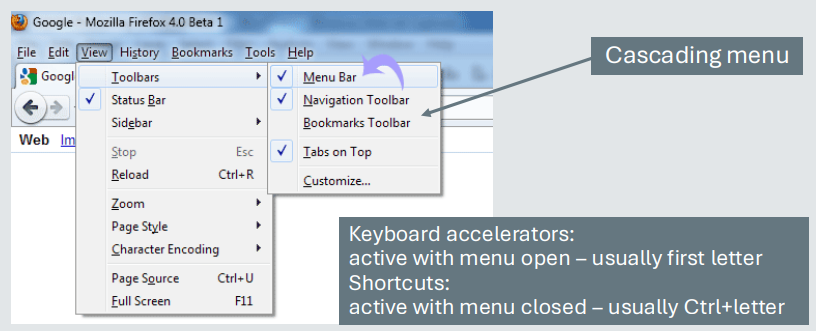
\includegraphics[width=\linewidth]{menu_bars.png}
\end{figure}

\subsubsection{Contextual Menu}
Contextual menu appears where you are\\
• pop-up menus - actions for selected object\\
• pie menus - arranged in a circle\\
- easier to select item (larger target area)\\
- quicker (same distance to any option)

\begin{figure}[h!]
  \centering
  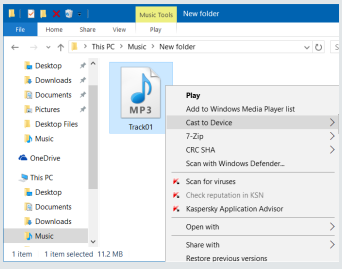
\includegraphics[width=\linewidth]{context_menu.png}
\end{figure}

\subsubsection{Menus design issues}
Menus are hidden most of the time

• Which kind to use\\
• What to include in menus\\
• Words to use (action or description)\\
• How to group items\\
• Choice of keyboard accelerators

\subsubsection{Other WIMP components}
Buttons\\
individual and isolated regions within a display that can be selected to invoke
an action (include radio buttons and check boxes)

Toolbars\\
long lines of icons that give quick access to common actions

Palettes\\
little windows of actions (e.g. available shapes in drawing package)

Tear-off menus\\
a menu can tear off to become a palette

Dialogue boxes\\
information windows that pop up to inform of an important event or request information

\chapter{Lecture 2 - Perception and cognition in design}

Low level perception – what visual characteristics effect how well we
can perceive the contents of a display?

Attention – how can displays help/hinder our ability to be aware
of relevant information?

Memory – how challenging are the requirements of the interface?\\

Outline of perception and cognition (simplified diagram of human information processing);
\begin{figure}[h!]
  \centering
  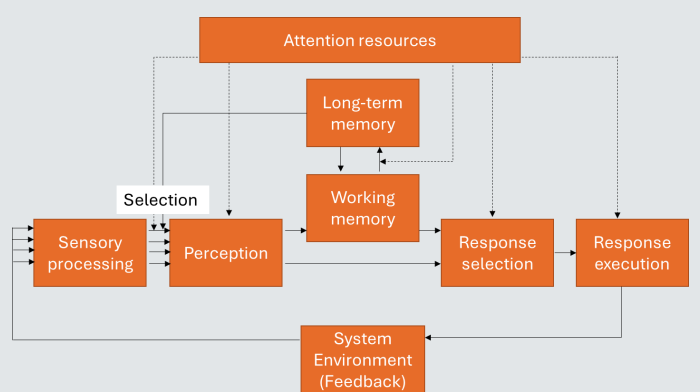
\includegraphics[width=\linewidth]{outline_perception_and_cognition.png}
\end{figure}

Starting with sensory processing, our retinas respond to light, our hair cells in the
air are being vibrated by sound, etc. We don't necessarily perceive all of these.

What makes it to conscious perception is limited by attention resources during
selection. As we are perceiving the world, we are immediately holding that information
in our working memory (short-term memory).

If you hold things in your working memory for long enough, it will make it into
your long-term memory. Long term memory can also feed back into the selection
process, producing a bias in what is perceived.

We can manipulate our working memory to think about what we are going to do next;
response selection. Then we can carry out that task; response execution.

Attention resources limit all of these, so you can't be distracted,
thinking about something else, while trying to form and execute a response.

After the execution of a response, a change occurs in the environment, creating a
loop as it produces new sensory input.

\section{Visual Acuity}
Acuity; Visual resolution - the smallest object you can see

\subsubsection{Vernier Acuity}
A way of measuring the smallest thing people can see\\
Testing if you can see the offset between two lines
\begin{figure}[h!]
  \centering
  
\includegraphics[width=1em]{vernier_acuity.png}
\end{figure}

\subsubsection{Landolt C}
Another way of measuring visual resolution
\begin{figure}[h!]
  \centering
  
\includegraphics[width=5em]{landolt_c.png}
\end{figure}

\subsubsection{Snellen Chart}
count how many letters you can read, without making a mistake
\begin{figure}[h!]
  \centering
  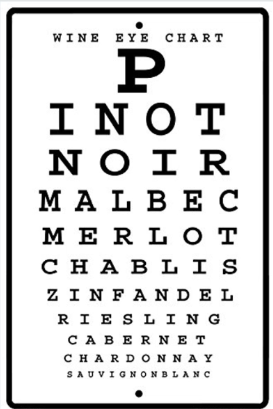
\includegraphics[width=10em]{snellen_chart.png}
\end{figure}

\newpage

\subsection{Foveal vs peripheral location}
Foveal location - looking right at it\\
Peripheral location - what you can see on the edge of your vision

Your peripheral vision is always worse at seeing things, this is
due to the structure of the eye;

Light is focused in one way, on the fovea. The fovea has the cones
(photoreceptors) responsible for high resolution color vision.

In your periphery, the cones are more spread out - lower resolution vision.
\begin{figure}[h!]
  \centering
  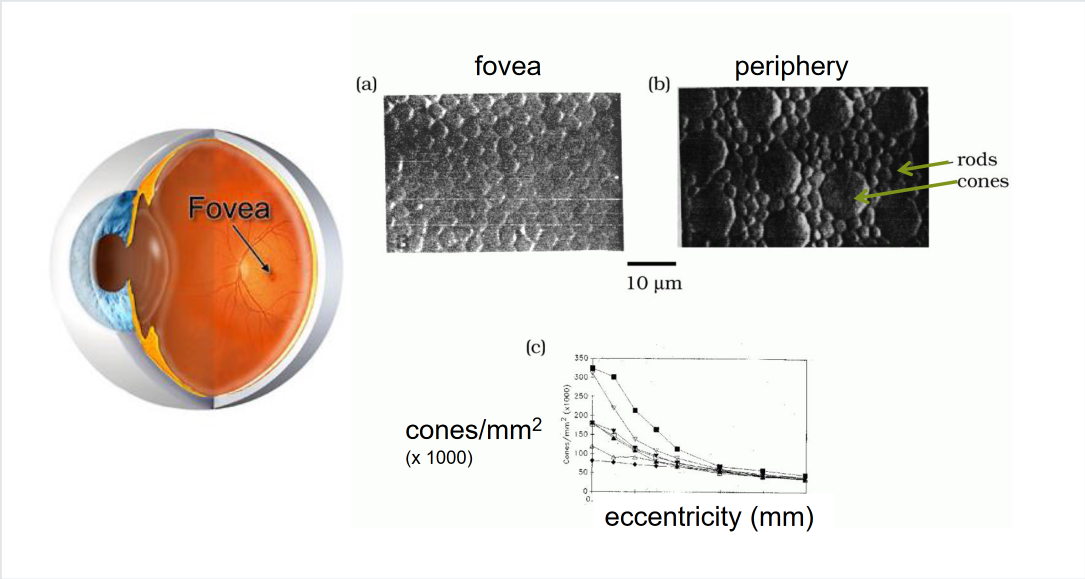
\includegraphics[width=\linewidth]{eye_structure.png}
\end{figure}

Even with people who have glasses or have had laser surgery, visual acuity
does drop off with age.

magnification factor - How much larger something needs to be presented in the periphery to be seen as clearly as in the fovea.

\subsection{Brightness and contrast}
Brightness - how much light is coming off the screen at a point

Contrast - the difference between the brightest point and darkest point
on the screen

Our brain is more sensitive to contrast - the visually impaired seem to
need larger UI but they also need higher contrast.

There is some evidence that dyslexics are over-sensitive to high-contrast images.

\newpage

\subsection{Color}

Color discrimination - we can distinguish between hue, saturation and luminance

Sometimes hue can win over low contrast, e.g., \colorbox{yellow}{when highlighting some text}

\subsubsection{Color blindness}

The most common form occurs in men and leads to difficulties in seeing differences
between red and green

8\% of men and 0.5\% of women have  the common form of red-green color blindness

CVD - color vision deficiency

\subsubsection{Color contrast and similarity}
We have 3 different types of photoreceptors

M cells respond the most to green wavelengths of light, whereas L cells respond
the most to red wavelengths of light. The most common cause of color-blind people
is them lacking L and M cells.

\begin{figure}[h!]
  \centering
  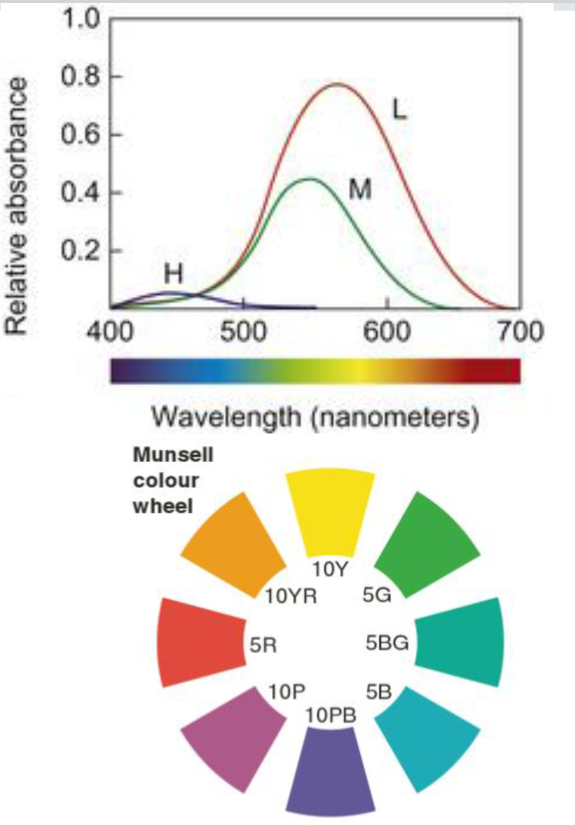
\includegraphics[width=20em]{color_contrast_and_similarity.png}
\end{figure}

The wheel captures similarity between colors.

\subsection{Movement}
Motion threshold – Humans are very sensitive to motion, very small displacements
can be detected.

Flicker and motion onset/offset can be used to attract attention.

\subsubsection{Apparent motion}
For the sense of apparent motion an object needs to change location\\
good enough for the brain\\
e.g., animated movies

Dmin is defined as the minimum distance over which spatial change is seen
as motion (if something moves too little you won't detect it)

Dmax is the maximum spatial gap over which motion is seen (if something moves too
far, you may not see it as the same object, but one disappearing and another appearing
somewhere else)

Similary, there is a limit on time. You won't detect motion if there is too small
or too large of a gap

Dmin can be as low as 0.01deg, Dmax can be many degrees of visual angle for moving
objects

\subsubsection{Attention in displays}
Attention is a limited resource

Attention can be thought of as a ‘bottle-neck’ of processing.

We do not take in all that is presented in the scene at any given time.

The visual attributes above need to be considered along with what the other objects
in the display are and what the task is.

Visual attention is usually closely linked with where the eyes are looking
– can use eye tracking as measure

Selective visual attention - how do we decide what to pay attention to?\\
1. General orientation and scene scanning\\
2. Supervisory control, e.g., driving\\
3. Noticing - breaking attention\\
4. Searching\\
5. Reading - requires a special kind of attention\\
6. Confirming

Salience - how much an object stands out against a background\\
Displays increase salience when trying to attract attention

\newpage

\begin{figure}[h!]
  \centering
  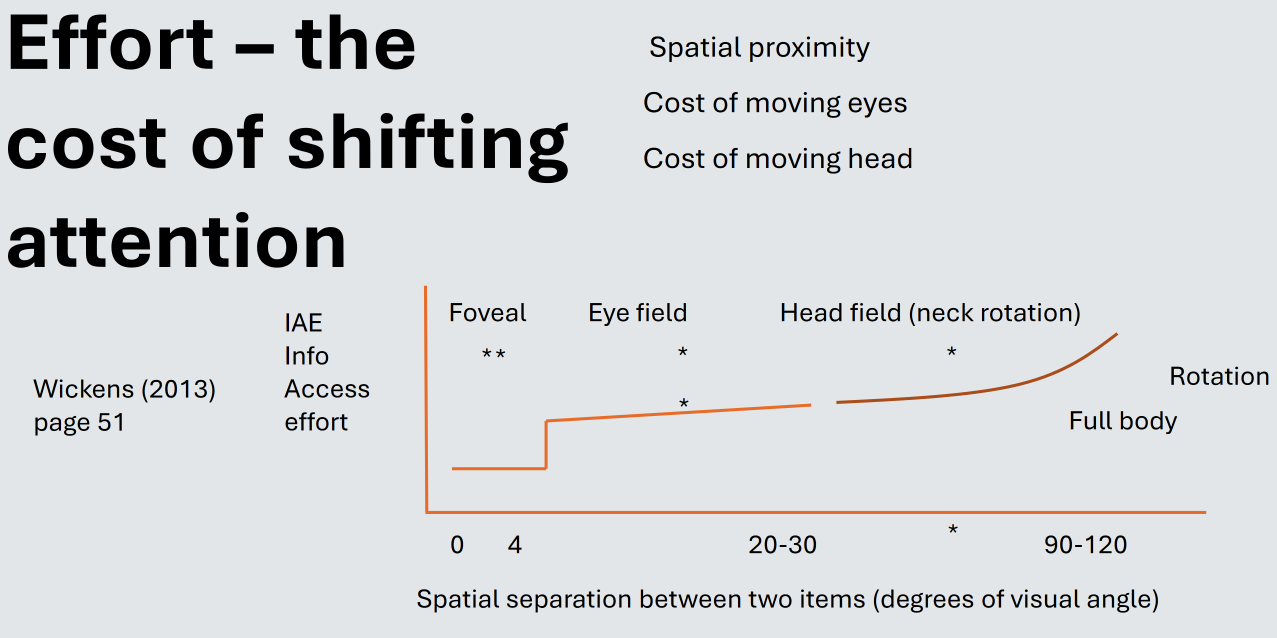
\includegraphics[width=\linewidth]{the_cost_of_shifting_attention.png}
\end{figure}

\subsubsection{Task relevance, Expectancy, \& Noticing}
Can be defined positively (the value or relevance of information for a task).\\
Or negatively (e.g. the cost of missing a warning).

At any point in time we may have many tasks, the more highly weighted ones may
override the others.

Attention can be guided to areas where information is rapidly changing\\
(e.g. curvy road edges attract more attention than straight).

Our prior experience may guide our attention to where we expect information to
be. Contextual cues (see later) such as arrows lead to expectation and thus guide
attention.

Although the human visual systems is usually sensitive to change, sometimes we
fail to see changes. Inside the lab this is called \textbf{change blindness}.

Can be caused by some sort of visual interruption, such as an eye movement at the
the wrong time.

\subsubsection{Search}
Visual search is a useful paradigm for examining the mechanisms of attention.\\
Some features ‘pop out’, some need ‘serial search’.\\
It is also a real-life task when looking at a display.

A signature of serial search is "search time increases with the number of distractors"

A signature of pop out is "search time does not increase with the number of distractors"

\newpage

Serial search;
\begin{figure}[h!]
  \centering
  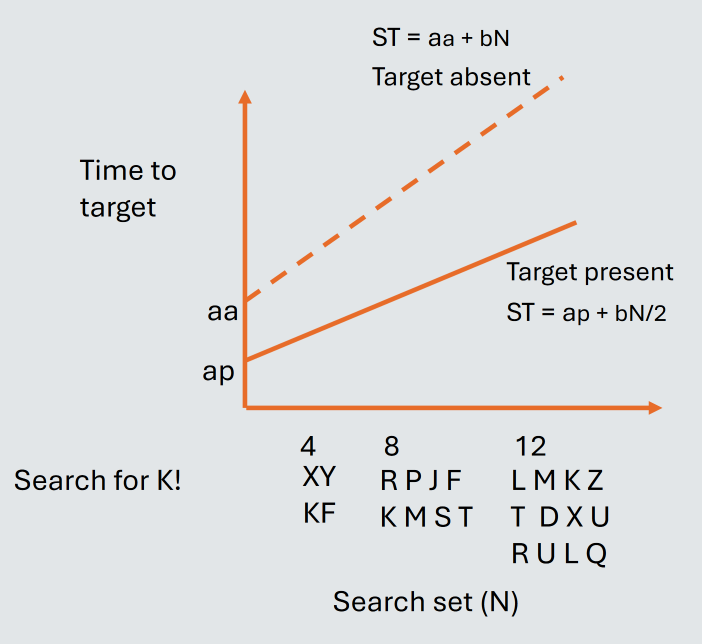
\includegraphics[width=\linewidth]{serial_search_absent_present_target.png}
\end{figure}

It takes us about half the time to find a letter than it does to work out
that it is not there (since we have to look through all letters and we
tend to check back a bit)

\subsubsection{Clutter}
This is a term closely related to search, given a certain target describes how
the rest of the contents of the display impede visual search.

Numerosity clutter - too many other objects.

Proximity or readout clutter - too many nearby objects, hence local and global
density clutter is also often referred to.

Disorganizational clutter - lack of spatial structure in the background objects
can interfere.

Heterogeneous clutter – many different distractors make search difficult.

\subsubsection{Directing and guiding attention}

Central cue - cue attention by making use of where someone is looking already\\
E.g., arrows have been shown to automatically guide attention

Peripheral cue - something that you are not looking at right now but they grab
your attention from the edge of your vision\\
By making things become salient they can catch attention.\\
An example of this is highlighting in a display – but this has to not obscure the
area of interest.

\subsubsection{Working memory}
We must design with the mind in mind

Working memory - Temporary attention demanding store, used to store information
before we use it or combine different bits of information.

Closely related to attention – e.g. in visual search we are looking for a target
that we are holding in working memory.

Failures occur in a work context, for example carrying out a list of tasks,
checking a list, remembering a procedure.

Lab measures:
digit span, word span, reading span, operation span (doing some math, etc.),
counting span.

The measures correlate with real world human performance in tasks such as\\
reading and listening comprehension,\\
academic performance, multi-tasking,\\
language comprehension, ability to follow\\
directions, vocabulary learning, note taking,\\
writing, reasoning, learning to programme,\\
making complex aviation decisions

\newpage

\begin{figure}[h!]
  \centering
  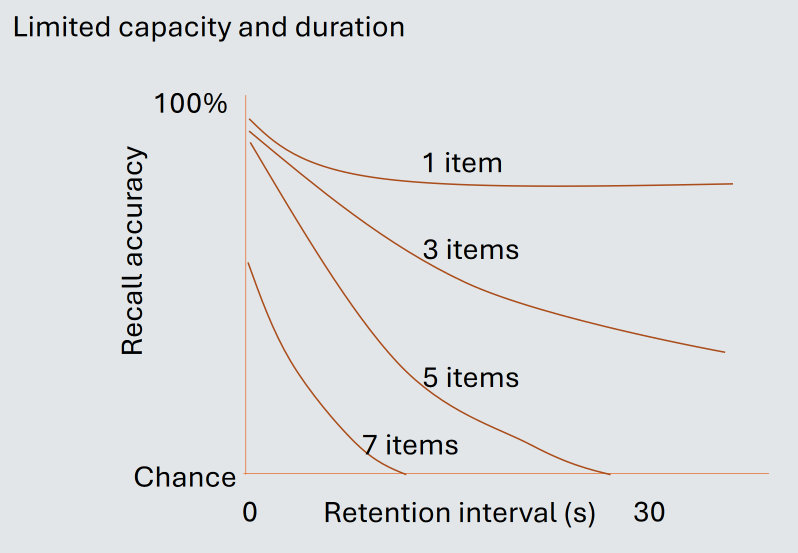
\includegraphics[width=\linewidth]{working_memory_decay_graph.png}
\end{figure}
The more things you are trying to hold in memory, the more quickly they disappear

Similar decay curves found for navigational information and information
used by radar controllers.

7 is a good number of things we can remember; magic number of 7 +/- 2

\textbf{Interference and confusion}

information doesn't disappear due to simplly fading, but instead it's due
to new information coming in.

Having to carry out another task whilst holding items in memory will interfere with
the ability to recall the original items (retroactive interference) but can also
affect memory for new items (proactive interference)

\newpage

Example of a lab measure;
\begin{figure}[h!]
  \centering
  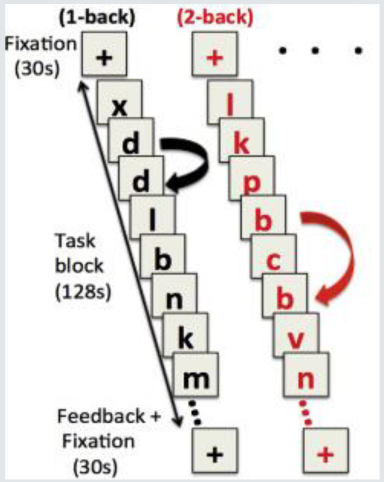
\includegraphics[width=20em]{1_back_2_back_lab_measure.png}
\end{figure}
You ask the individual if a letter has appeared more than once within a 1 letter gap\\
You then do the same but for a 2 letter gap - 2-back is enough to show differences in age;
\begin{figure}[h!]
  \centering
  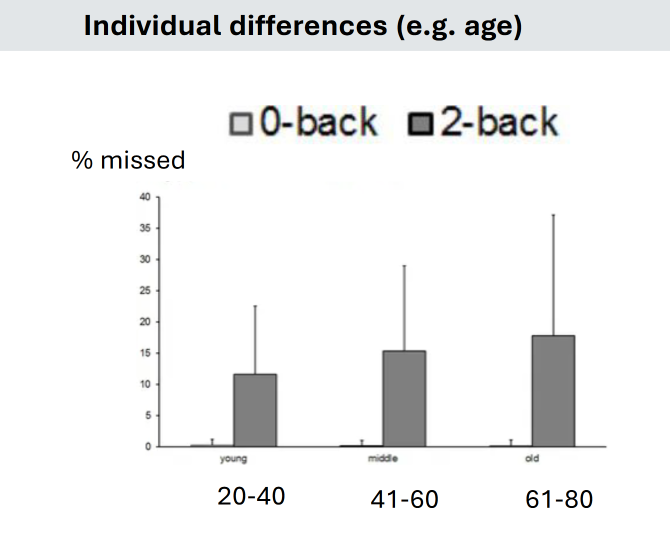
\includegraphics[width=\linewidth]{working_memory_1_back_age_differences.png}
\end{figure}

\chapter{Workshop 2}
Gestalt psychology described the principles that makes us visually group objects
together
\begin{figure}[h!]
  \centering
  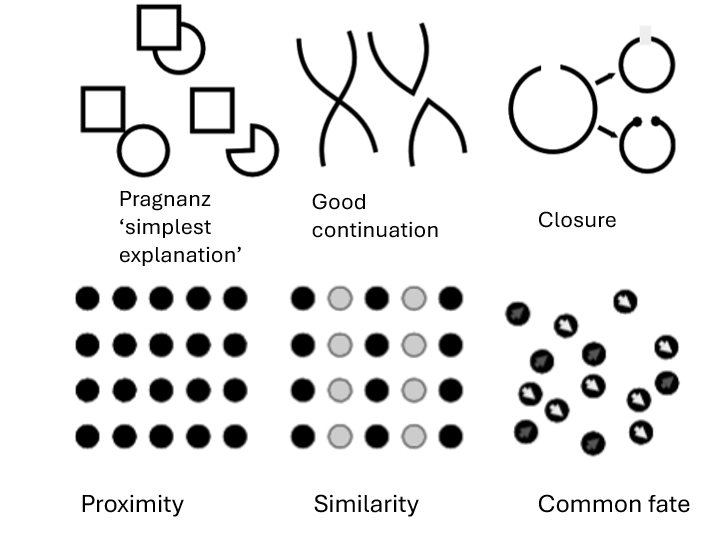
\includegraphics[width=\linewidth]{gestalt_psychology_group_objects_principles.png}
\end{figure}

\textbf{Bottom-up (exogenous) attention} \\
- Stimuli that attract your attention

\textbf{Top-down (endogenous) attention}\\
- Stimuli that you are focussing your attention on

\textbf{Inattentional blindness}\\
even when something  is very salient it can go unnoticed \\
attending to a spatial location or feature makes us blind to salient parts of the display

Difficulty of primary task with degree of visual similarity between unexpected task and primary event.

E.g., Look, but fail to see reported in driving\\
Needs to be considered if you want people for example to pay attention to a warning on an interface.

Spatial memory is limited and can easily becomes overburdened.\\
Time and interference affect memory.

\chapter{Lecture 3 - Interaction Design \& Usability}
Three categories of things to keep in mind when designing for maximum usability;\\
\bulletPoint Principles to support usability - general understanding of the system\\
\bulletPoint Standards and guidelines - directions for the system design\\
\bulletPoint Design patterns - capture and reuse design knowledge

The first two categories are design rules

\section{Principles to support usability}
Learnability - How easy is it to interact with the system?

Flexibility - Are there multiple ways of interaction?

Robustness - Is the system reliable?\\
Is the internal state of the system perceivable from its representation?

\subsection{Learnability}
The ease with which new users can begin effective interaction and achieve maximal
performance\\
\bulletPoint Predictability\\
\bulletPoint Synthesizability\\
\bulletPoint Familiarity\\
\bulletPoint Generalizability\\
\bulletPoint Consistency

\subsubsection{Predictability}
Support for the user to determine the effect of future actions based on past
interaction history\\
\bulletPoint operation visibility\\
\bulletPoint the same sequence of actions will always trigger the same results

This helps give confidence to the user about the robustness of the software

\newpage

Examples;
\begin{figure}[h!]
  \centering
  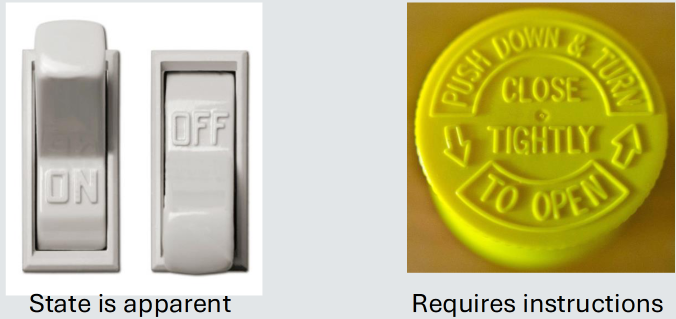
\includegraphics[width=20em]{predictability_examples.png}
\end{figure}
The lid on the right is unlike other lids and so requires special instructions to be
written at the top - like a mini manual

The switches on the left are a lot better but still have issues. Does "ON" mean
the system is on or does it mean that it will turn on once you flick it in that
direction?

\subsubsection{Synthesizability}
Support for the user to assess the effect of past operations on the current state

Example;
\begin{figure}[h!]
  \centering
  
\includegraphics[width=\linewidth]{synthesizability_example.png}
\end{figure}
Why two 'Shipping' states? Maybe needs confirmation. At least the user knows
there are 4 states, instead of 3.

\subsubsection{Familiarity}
The extent to which a user’s knowledge and experience in other real-world or
computer-based domains can be applied when interacting with a new system

\begin{figure}[h!]
  \centering
  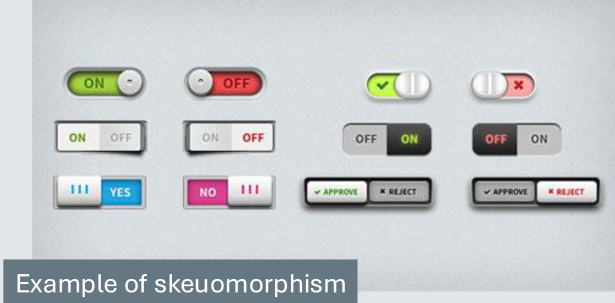
\includegraphics[width=\linewidth]{familiarity_example.png}
\end{figure}
Not perfect but better than what was seen before. The color of the switches
tell you the status of the system, but it may not be accessible to, e.g.,
color-blind people.

\newpage

\subsubsection{Generalizability}
Support for the user to extend knowledge of specific interaction within and across
applications to other similar situations\\
\bulletPoint similar icons and buttons\\
\bulletPoint similar menu structure

E.g., floppy disk icon for save operations or title bar menus (File, Edit, View, Tools, etc.)

\subsubsection{Consistency}
Likeness in input-output behaviour arising from similar situations
or similar task objectives\\
\bulletPoint in a text editor, "save", "save as" and "export" have similar behaviours\\
\bulletPoint  the printing mechanism is similar across applications and systems

\subsection{Flexibility}
The multiplicity of ways the user and system exchange information\\
\bulletPoint Dialogue initiative\\
\bulletPoint Task migratability\\
\bulletPoint Substitutivity\\
\bulletPoint Multithreading\\
\bulletPoint Customisability

You can sometimes assume that a user has some level of experience with your
UI and so it will be useful to give them flexibility - system tailors the UI to them
or let them tailor it to themselves

\subsubsection{Dialogue initiative}
Protecting the user freedom from artificial constraints on the input dialog
imposed by the system\\
\bulletPoint System preemptiveness vs. user preemptiveness

The system may need to take the initiative and tell the user some information,
instead of forcing users to lead the initiative

Example;
\begin{figure}[h!]
  \centering
  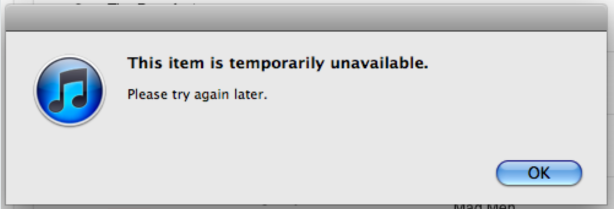
\includegraphics[width=\linewidth]{dialog_initiative_example.png}
\end{figure}

\newpage

\subsubsection{Task migratability}
The ability to pass control for the execution of a given task so that it becomes
either internalized by the user or the system or shared between them

Example;
\begin{figure}[h!]
  \centering
  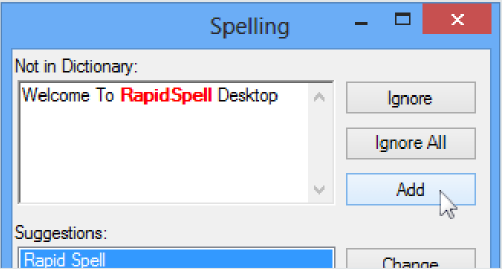
\includegraphics[width=\linewidth]{task_migratability_example.png}
\end{figure}

There is a collaboration between the system and the user to achieve a task. E.g.,
here you trigger it, the system then controls it and gives you suggestions,you
then respond, etc.

\subsubsection{Substitutivity}
Allowing equivalent values of input and output to be arbitrarily substituted
for each other\\
\bulletPoint Representation multiplicity (keyboard shortcuts, different locations
for the same actions)
\bulletPoint Equal opportunity for users (who choose different options)

Example;
\begin{figure}[h!]
  \centering
  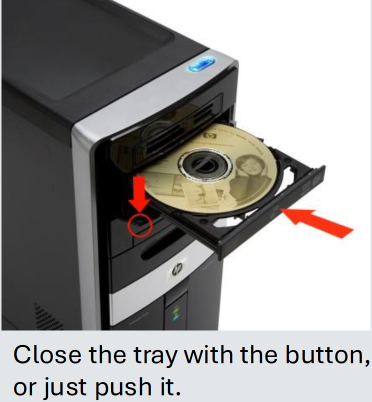
\includegraphics[width=15em]{substitutivity_example.png}
\end{figure}

Provide a good level of control for experienced users - allow them to optimize their workflow

\subsubsection{Multithreading}
Ability of the system to support user interaction pertaining to more than one
task at a time\\
\bulletPoint Concurrent interaction\\Using a browser window while another one
loads or Editing several documents at the same time\\
\bulletPoint Multimodality\\
The system has multiple ways of communicating its state
(e.g. simultaneous image and sound)
and several modes of interaction
(e.g. simultaneous typing and voice)

\subsubsection{Customisability}
adaptability - Modifiability of the user interface by the user\\
adaptivity - Modifiability of the user interface by the system

E.g., AutoCAD software - moving toolbars, hiding them in the shelves, saving workspaces, etc.
\begin{figure}[h!]
  \centering
  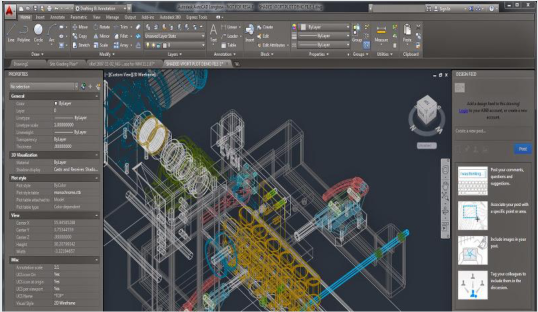
\includegraphics[width=15em]{customisability_example.png}
\end{figure}

\subsection{Robustness}
The level of support provided to the user in determining successful achievement
and assessment of goal-directed behaviour\\
\bulletPoint Observability\\
\bulletPoint Recoverability\\
\bulletPoint Interaction responsiveness\\
\bulletPoint Task conformance

\subsubsection{Observability}
Ability of user to evaluate the internal state of the system from its perceivable
representation\\
\bulletPoint Browsability\\
\bulletPoint Default settings\\
\bulletPoint Reachability\\
\bulletPoint Persistence\\
\bulletPoint Operation visibility

\newpage

Example;
\begin{figure}[h!]
  \centering
  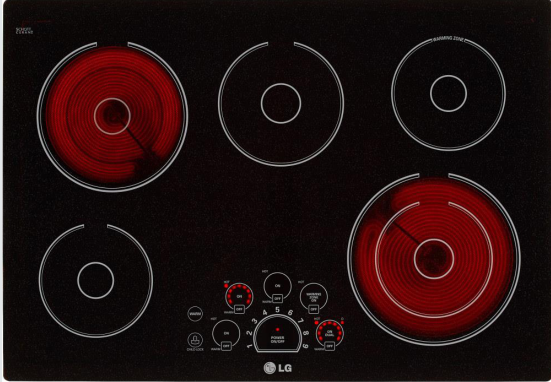
\includegraphics[width=15em]{observability_example.png}
\end{figure}

\subsubsection{Recoverability}
Ability of user to take corrective action once an error has been recognized\\
• Reachability and forward/back recovery\\Undo buttons, undo history\\
• Commensurate effort\\
If an action is difficult to undo then it should have been
difficult to do in the first place.\\
Conversely, easily undone actions should be easy to do.

Example;
\begin{figure}[h!]
  \centering
  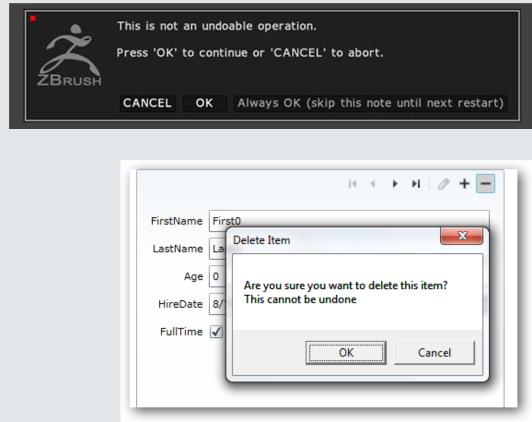
\includegraphics[width=15em]{recoverability_example.png}
\end{figure}

\subsubsection{Interaction responsiveness}
How the user perceives the rate of communication with the system\\
• stability\\
• speed

Bad Example - you don't know what is happening anymore (is it frozen?);
\begin{figure}[h!]
  \centering
  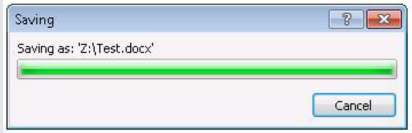
\includegraphics[width=15em]{interaction_responsiveness_example.png}
\end{figure}

\newpage

\subsubsection{Task conformance}
The degree to which the system services support all of the tasks the user
wishes to perform, in a way that the user understands them\\
• task completeness\\
• task adequacy

\section{Principles, Standards and Guidelines}
Principles are abstract rules\\
\bulletPoint Principles to support usability\\
\bulletPoint Psychology\\
\bulletPoint Computer Science\\
\bulletPoint Other areas of study\\
Guidelines recommend best practices\\
\bulletPoint Fonts and colour schemes in commercial software\\
\bulletPoint Accessibility in personal blog\\
\bulletPoint Size of buttons in web app\\
Standards are policies\\
\bulletPoint Fonts and colour schemes in aviation software\\
\bulletPoint Accessibility in governmental websites\\
\bulletPoint Size of emergency button on medical devices

Authority of a rule\\
Indication of whether the rule should be followed, or if it is only a suggestion

Generality of a rule\\
Indication of whether the rule can be applied to many design situations,
or if it is specific to an application

Principles – abstract design rules\\
\bulletPoint low authority\\
\bulletPoint high generality\\
\bulletPoint Set by broad disciplines related to interaction\\
\bulletPoint Based on research and experience\\
\bulletPoint Applicable principles\\
\bulletPoint First principles

Guidelines – general design rules\\
\bulletPoint medium authority\\
\bulletPoint medium generality\\
\bulletPoint More suggestive and general\\
\bulletPoint Many textbooks and reports full of guidelines\\
\bulletPoint General guidelines (principles) applicable during early life cycle activities\\
\bulletPoint Detailed guidelines (style guides) applicable during later life cycle activities\\
\bulletPoint Understanding justification for guidelines aids in resolving conflicts

\newpage

Standards – specific design rules\\
\bulletPoint high authority\\
\bulletPoint limited application\\
\bulletPoint Set by national or international bodies to ensure compliance by a large community of designers\\
\bulletPoint Require sound underlying theory and slowly changing technology\\
\bulletPoint Regulations can reinforce mandatory compliance\\
\bulletPoint Hardware standards more common than software ones (usually have high authority and low level of detail)\\
\bulletPoint ISO 9241 defines usability as effectiveness, efficiency and satisfaction with which users accomplish tasks

\chapter{Workshop 3 - Usability}
Usability is a quality attribute that assesses how easy user interfaces are to
use. The word "usability" also refers to methods for improving ease-of-use during
the design process.

Principles;\\
\bulletPoint Learnability\\
Can new users easily understand how to perform basic tasks?\\
\bulletPoint Efficiency\\
Are returning users able to perform their tasks with good timing?\\
\bulletPoint Memorability\\
How easy is it for users to remember how the system works, even after not using
it for a significant amount of time?\\
\bulletPoint Errors\\
How frequently do users incur in errors, and how serious are these? Is it possible to
recover from errors?\\
\bulletPoint Satisfaction\\
Is it pleasant to use the design?

Usability can be applied to any type of interface\\
Eventhough many examples are on software user interfaces\\
For example, Web pages

Evaluation;\\
The most common method is user testing

Jakob Nielsen, one of the pioneers in the field stated that five users are all it typically
takes to find most usability problems in an interface\\
- this does not exclude large scale studies to fine tune design and impact.

Testing multiple times allows constant improvement\\
This can follow a progression from low-fidelity prototypes (e.g. UI drawings) to full
applications

\section{Heuristic Evaluation}
Heuristic; Technique based in past experience that can assist at arriving a solution
for a problem

Heuristic evaluation;\\
\bulletPoint Use of heuristics to determine (and sometimes quantify) quality\\
\bulletPoint Informal, but useful mechanism\\
\bulletPoint Experts examine an interface and evaluate it against a set of principles

A single usability heuristic may address more than one usability principle.

\newpage

\subsection{Nielsen’s Usability Heuristics}
Several sets of usability heuristics exist, the most well-known and used being Nielsen’s\\
\bulletPoint Visibility of system status\\
\bulletPoint Match between system and the real world\\
\bulletPoint User control and freedom\\
\bulletPoint Consistency and standards\\
\bulletPoint Error prevention\\
\bulletPoint Recognition rather than recall\\
\bulletPoint Flexibility and efficiency of use\\
\bulletPoint Aesthetic and minimalist design\\
\bulletPoint Help users recognize, diagnose, and recover from errors\\
\bulletPoint Help and documentation

\subsubsection{Visibility of system status}
The system should always keep users informed about what is going on, through
appropriate feedback within reasonable time

Example;
\begin{figure}[h!]
  \centering
  
\includegraphics[width=\linewidth]{visibility_of_system_status_example.png}
\end{figure}

\subsubsection{Match between system and the real world}
The system should speak the users' language, with words, phrases and concepts
familiar to the user, rather than system-oriented terms

Follow real-world conventions, making information appear in a natural and logical
order

Example;
\begin{figure}[h!]
  \centering
  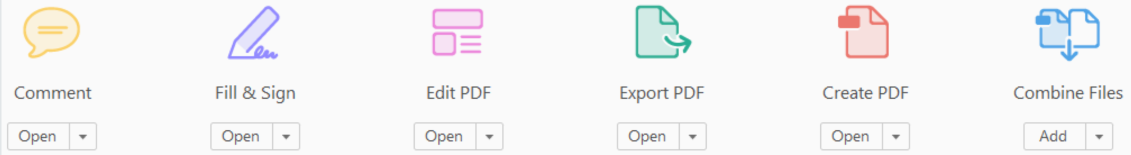
\includegraphics[width=\linewidth]{match_between_system_and_the_real_world_example.png}
\end{figure}

\newpage

\subsubsection{User control and freedom}
Users often choose system functions by mistake and will need a clearly marked
"emergency exit" to leave the unwanted state without having to go through an extended
dialogue

Support undo and redo

Example;
\begin{figure}[h!]
  \centering
  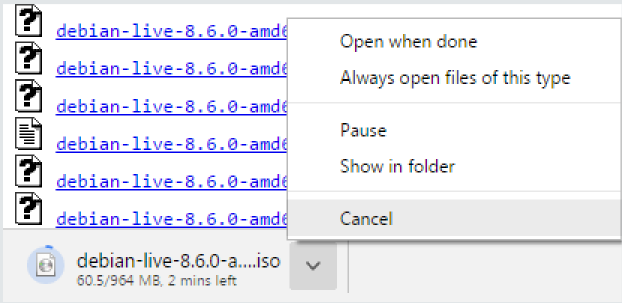
\includegraphics[width=\linewidth]{user_control_and_freedom_example.png}
\end{figure}

\subsubsection{Consistency and standards}
Users should not have to wonder whether different words, situations, or actions mean
the same thing - follow platform conventions

Example;
\begin{figure}[h!]
  \centering
  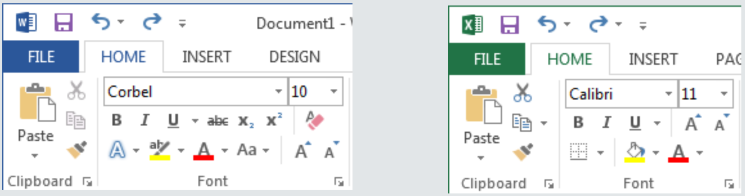
\includegraphics[width=\linewidth]{consistency_and_standards_example.png}
\end{figure}

\newpage

\subsubsection{Error prevention}
Even better than good error messages is a careful design that prevents a problem
from occurring

Either eliminate error-prone conditions or check for them and present users with a
confirmation option

Example;
\begin{figure}[h!]
  \centering
  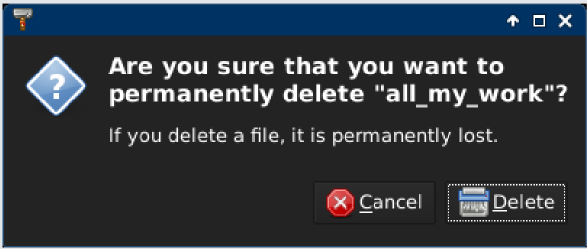
\includegraphics[width=20em]{error_prevention_example.png}
\end{figure}

\subsubsection{Recognition rather than recall}
Minimize the user's memory load by making objects, actions, and options visible

The user should not have to remember information from one part of the dialogue to
another

Instructions for use of the system should be visible or easily retrievable whenever
appropriate.

Example;
\begin{figure}[h!]
  \centering
  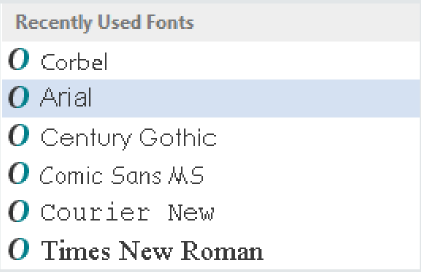
\includegraphics[width=20em]{recognition_rather_than_recall_example.png}
\end{figure}

The most relevant user interface elements should be visible to the user at each step of its use.

A user interface that is in line with this heuristic addresses some elements of the memorability principle.

\newpage

\subsubsection{Flexibility and efficiency of use}
Accelerators (unseen by novice users) may often speed up the interaction for expert users\\
Allow users to tailor frequent actions

Example;
\begin{figure}[h!]
  \centering
  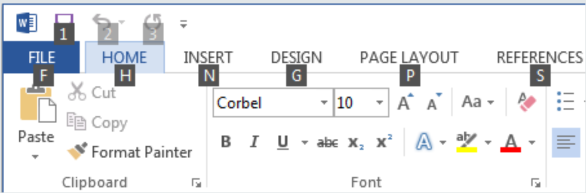
\includegraphics[width=20em]{flexibility_and_efficiency_of_use_example.png}
\end{figure}

\subsubsection{Aesthetic and minimalist design}
Dialogues should not contain information which is irrelevant or rarely needed

Every extra unit of information in a dialogue competes with the relevant units of
information and diminishes their relative visibility

Example;
\begin{figure}[h!]
  \centering
  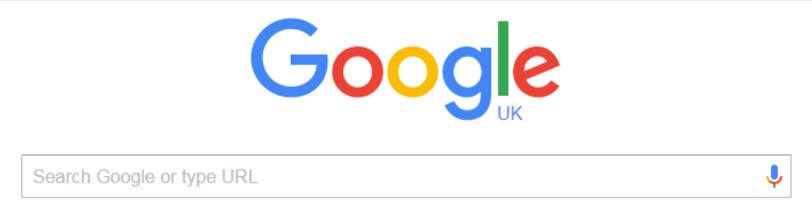
\includegraphics[width=\linewidth]{aesthetic_and_minimalist_design_example.png}
\end{figure}

\newpage

\subsubsection{Help users recognize, diagnose, and recover from errors}
Error messages should be expressed in plain language (no codes), precisely
indicate the problem, and constructively suggest a solution

Example;
\begin{figure}[h!]
  \centering
  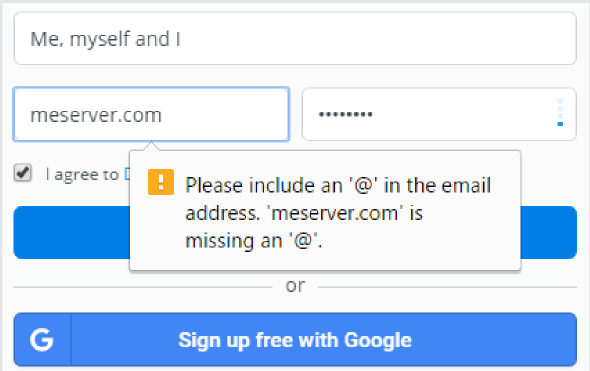
\includegraphics[width=20em]{help_users_recognize_diagnoze_and_recover_from_errors_example.png}
\end{figure}

\subsubsection{Help and documentation}
Even though it is better if the system can be used without documentation, it may be
necessary to provide some help and documentation

Any such information should be easy to search, focused on the user's task, list
concrete steps to be carried out, and not be too large

Example;
\begin{figure}[h!]
  \centering
  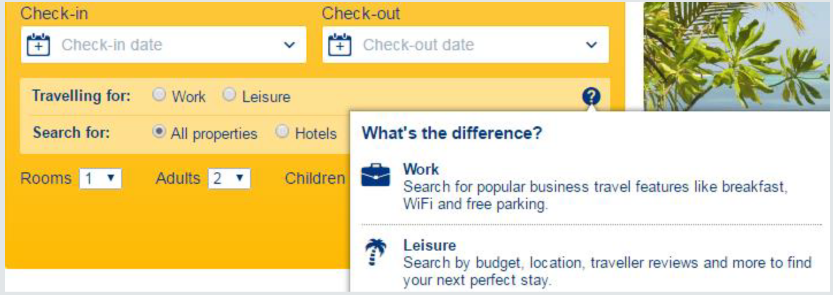
\includegraphics[width=\linewidth]{help_and_documentation_example.png}
\end{figure}

\chapter{Lecture 4 - Graphic Design}

Appearance (graphic design) + Behavior (interaction design) = look and feel

Graphic design is problem solving relating to visual communication

\section{Typography (fonts, readability of text)}

\begin{figure}[h!]
  \centering
  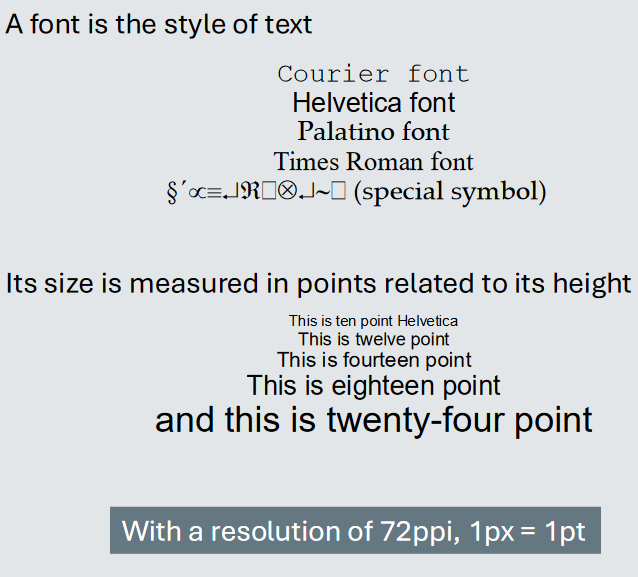
\includegraphics[width=\linewidth]{fonts.png}
\end{figure}

\newpage

Pitch is the horizontal space a font takes up\\
• monospace: every character has the same width - used where alignment matters (e.g., in an IDE)
\begin{figure}[h!]
  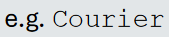
\includegraphics[width=6em]{courier_font.png}
\end{figure}

• proportional: some characters are wider than others - what we normally use to read
\begin{figure}[h!]
  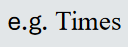
\includegraphics[width=5em]{times_font.png}
\end{figure}

\begin{figure}[h!]
  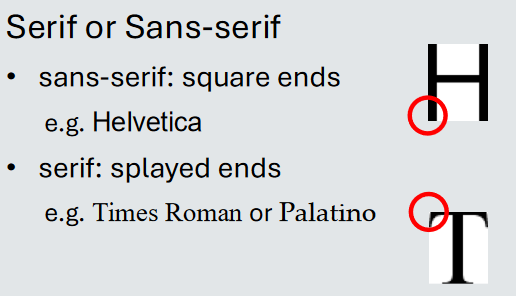
\includegraphics[width=20em]{serif_sans_serif_fonts.png}
\end{figure}

Sans serif is normally used for titles, with books normally using fonts with serif.

\begin{figure}[h!]
  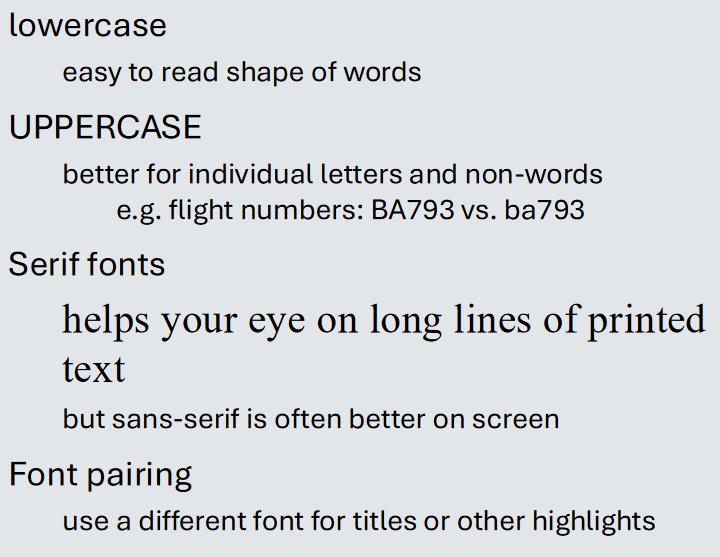
\includegraphics[width=20em]{readability_of_text.png}
\end{figure}

In general simplicity and having contrasts is best\\
Don't use more than 2 or 3 fonts (e.g., one for titles, one for body text, one for display text)\\
Use different styles (\textit{italic}, \textbf{bold}, etc.) to establish essential contrasts\\
Copy font combinations that are widely used

Only print something if you really have to, and not in color unless it is essential\\
color cartridges for printers are very bad for the environment\\
Font choice can have an impact on the number of pages you can print

\begin{figure}[ht!]
  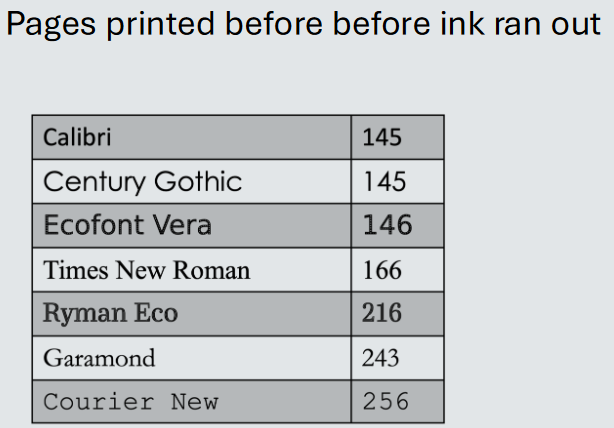
\includegraphics[width=20em]{pages_printed_before_ink_ran_out_fonts.png}
\end{figure}

\newpage

\section{Space (screen design and layout)}

Ask    - what is the user doing? (layout will always depend on this)

Think  - information, comparisons, order (organization of information dictates what the user will do with it, e.g., logos are always at the top since that is where everyone looks first, instead of at the bottom, on the right, in a small size)

Design - form follows function (if the functionality required is not available, then design is irrelevant)

\begin{figure}[ht!]
  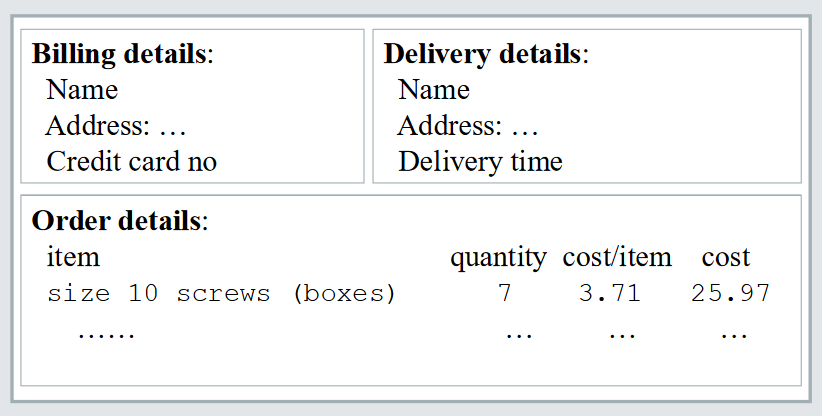
\includegraphics[width=40em]{graphic_design_grouping_items.png}
\end{figure}

place logically similar items, physically together

Start by understanding the natural order, it should match the screen order\\
• use boxes, space, etc.\\
• set up tabbing right\\

Instructions\\
beware the “cake recipe” syndrome\\
1. Mix milk and flour\\
2. Add the fruit after beating them\\
3. Add one egg yolk before the fruit

Use boxes to group logical items\\
Use fonts for emphasis, headings\\
But not too many of each

\begin{figure}[ht!]
  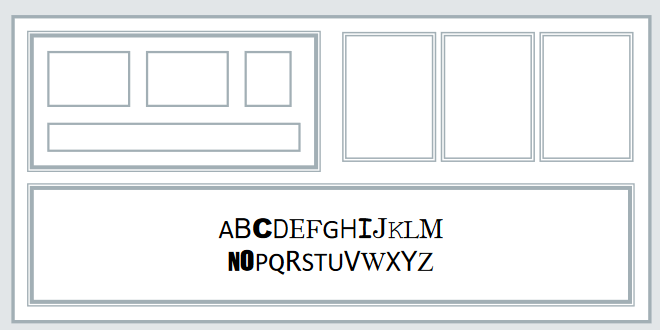
\includegraphics[width=40em]{graphic_design_decoration.png}
\end{figure}

If the text is read from left to right align it on the left-hand side

\begin{figure}[ht!]
  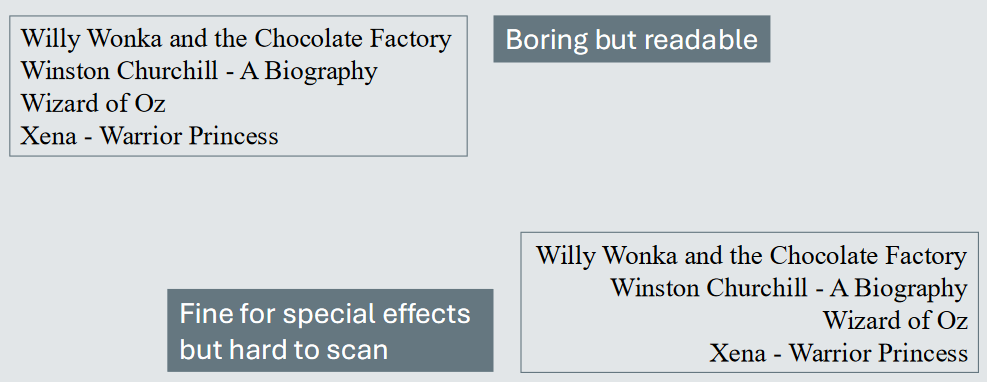
\includegraphics[width=40em]{graphic_design_text_alignment.png}
\end{figure}

We usually scan for surnames - highlight them with alignment

\begin{figure}[ht!]
  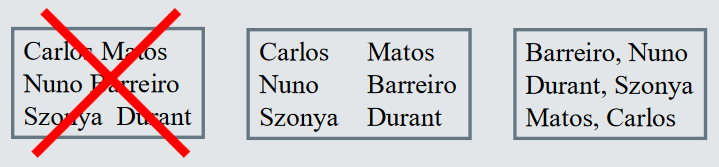
\includegraphics[width=40em]{graphic_design_surname_alignment.png}
\end{figure}

Visually, a long number is a big number\\
• align decimal points\\
• or right align integers


\begin{figure}
  \centering
  \begin{subfigure}{.5\textwidth}
    \centering
    \includegraphics[width=.7\linewidth]{graphic_design_bad_integers.png}
  \end{subfigure}%
  \begin{subfigure}{.5\textwidth}
    \centering
    \includegraphics[width=.7\linewidth]{graphic_design_good_integers.png}
  \end{subfigure}
\end{figure}

\newpage

Scanning across gaps is hard

\begin{figure}[ht!]
  \includegraphics[width=40em]{graphic_design_multiple_columns_bad.png}
\end{figure}

Use leaders

\begin{figure}[ht!]
  \includegraphics[width=40em]{graphic_design_multiple_columns_leaders.png}
\end{figure}

\newpage

or greying (vertical too)

\begin{figure}[ht!]
  \includegraphics[width=40em]{graphic_design_multiple_columns_greying.png}
\end{figure}

or even use ‘bad’ alignment (with care)

\begin{figure}[ht!]
  \includegraphics[width=40em]{graphic_design_multiple_columns_bad_alignment.png}
\end{figure}

In Typography, the space between letters is called the counter\\
Its shape is part of the composition of letters

\begin{figure}[ht!]
  \includegraphics[width=40em]{the_counter.png}
\end{figure}

\newpage

\begin{figure}
  \centering
  \begin{minipage}{.5\textwidth}

    use space to seperate
    \vskip5cm
    use space to structure
    \vskip5cm
    Space to highlight / focus attention

  \end{minipage}%
  \begin{minipage}{.5\textwidth}

    \includegraphics[width=.4\linewidth]{graphic_design_space_to_seperate.png}
    \vskip3cm
    \includegraphics[width=.4\linewidth]{graphic_design_space_to_structure.png}
    \vskip4cm
    \includegraphics[width=.4\linewidth]{graphic_design_space_to_highlight.png}

  \end{minipage}
\end{figure}

Use whitespace (e.g. leave margins around a body of text)

• Use a generous leading - Make sure the body of text is not overcrowded\\
(e.g. in CSS use line-height of 120%)

• Keep the text paragraphs narrow\\
(about 60-75 characters or 12-15 words, like in news papers)

\newpage

\section{Color (3D effects)}

\begin{figure}
  \centering
  \begin{subfigure}{.5\textwidth}
    \centering
    \includegraphics[width=\linewidth]{graphic_design_color_bg_bad1.png}
  \end{subfigure}%
  \begin{subfigure}{.5\textwidth}
    \centering
    \includegraphics[width=\linewidth]{graphic_design_color_bg_bad2.png}
  \end{subfigure}
\end{figure}

\includegraphics[width=\linewidth]{graphic_design_color_bg_good.png}

Color and 3d effects are both often used very badly!

Colour\\
• colour overused\\
• beware colour blindness\\
• use sparingly to reinforce other information

3D effects\\
• good for physical information and some graphs\\
• but not if overused (e.g. text in perspective, 3D pie charts)

\includegraphics[width=\linewidth]{graphic_design_bad_use_of_color.png}

Don't rely solely on colour distinctions (colour blindness is common)

Keep the colour design simple (use few colours weakly saturated)

Pick one colour and several shades of grey (safe choice)

Copy colour schemes from other interfaces

Be consistent with expectations: green for good, red for error, etc.

Sustainability with the dark mode/theme;\\
• background colour of the system and its apps from a light colour to black or dark grey\\
• text appears in a light colour, typically white\\
• in OLED screens at 30\%-50\% brightness level, it will save 3\%-9\% power\\
• in OLED screens at 100\% brightness, it will save around 39\% to 47\% power\\
• in LCD screens there is no difference

\section{General guidelines (images, icons, simplicity)}

\subsection{Simplicity via reduction}

Eliminate whatever isn’t necessary\\
1. decide what the design needs to convey\\
2. examine every element to decide whether it serves an essential purpose (label, colour, font, line weight)\\
3. remove it if it isn’t essential, even if it seems essential, try removing it anyway to see if the design falls apart

\includegraphics[width=0.5\linewidth]{graphic_design_reduction_icons.png}

Icons have been reduced to the bare essentials - no element can be removed
without destroying the meaning

\subsection{Simplicity via regularity}

For the essential elements that remain\\
• use a regular pattern\\
• limit inessential variation among elements

Use the same font, colour, line width, dimensions, orientation for multiple elements

Irregularities in the design will be magnified in the user’s eyes and assigned
meaning/significance

If the design is mostly regular, the highlighted elements will stand out better

\subsection{Simplicity via double-duty}

Combine elements

e.g., a scroll bar\\
• affords dragging\\
• indicates the position of the scroll window relative to the entire document\\
• indicates the fraction of the document displayed in the scroll window (how much of the document you are currently seeing, reflectd by the size of the scrollbar)

e.g., a window’s title bar\\
• label (+ if the file is saved or not)\\
• dragging handle\\
• window activation indicator\\
• location for window control buttons

\subsection{Balance and symmetry}
Choose an axis (usually vertical) and distribute elements equally around the axis
\begin{figure}
  \centering
  \includegraphics[width=0.7\linewidth]{graphic_design_balance_and_symmetry.png}
\end{figure}

\newpage

\subsection{Affordances}
take into account ...

For physical objects\\
• shape and size suggest actions (pick up, twist, throw)\\
• culture too (buttons ‘afford’ pushing, mug handle ‘affords’ grasping)

For screen objects\\
• a button-like object ‘affords’ mouse click\\
• a physical-like object suggests use

Culture of computer use\\
• icons ‘afford’ clicking\\
• or even double clicking (not like real buttons)

\subsection{The squint test}
Close one eye and squint the other, to disrupt your focus

Contrasts communicate information or highlight elements.

The squint test simulates early visual processing, and is a
technique used to see whether the contrasts you’ve tried
to establish are readily apparent.

\subsection{Accessible Design}
Help people that live with\\
• Colour blindness\\
• Visual impairments\\
• Neurodiversity\\
• Autism\\
• Dyslexia\\
• etc.

\chapter{Workshop 4 - Task Analysis}

Task Analysis is the study of the way people perform tasks
with existing systems (not necessarily
computer-based)

Methods to analyse people's jobs:\\
• what people do\\
• what things they work with\\
• what they must know

The goal is to inform the design of new
systems, make improvements over existing
systems, or produce documentation

Approaches to task analysis;\\
Task decomposition\\
• splitting task into (ordered) subtasks\\
Knowledge-based techniques\\
• what the user knows about the task and how it is organised\\
Entity-relation based analysis\\
• relationships between objects, actions and the people who perform them

Generally you observe, collect unstructured lists of words and actions and then organise them using notation or diagrams

\begin{center}
  Systems analysis vs. Task analysis\\
  system design - focus - the user

  Cognitive models vs. Task analysis\\
  internal mental state - focus - external actions\\
  practiced ‘unit’ task - focus - whole job
\end{center}

\section{Task Decomposition}

Aims:\\
• describe the actions people do\\
• structure them within task-subtask hierarchy\\
• describe order of subtasks

Hierarchical task analysis (HTA) is one of
the approaches - its outputs are:\\
• a hierarchy of tasks and subtasks\\
• plans describing in what order and under what
conditions subtasks are performed.

\newpage

\subsection{Textual HTA description}
Note that only the plans denote order

example:
\includegraphics[width=\linewidth]{textual_HTA_description.png}

To generate the hierarchy;\\
1. Get list of tasks\\
2. Group tasks into higher level tasks\\
3. Decompose lowest level tasks further

Stopping rules\\
• How do we know when to stop?\\
• Is “empty the dust bag” simple enough?\\
• Purpose: expand only relevant tasks\\
E.g. P x C rule: P = prob. of a mistake, C = cost of mistake\\
• Motor actions: lowest sensible level

\subsection{Diagrammatic HTA}

HTA diagrams start from a top-level task, which is then decomposed in subtasks.

Tasks (and subtasks) are represented as rectangles with an internal label.

The diagrams are read top-down, with the hierarchy relationships shown as a vertical
line from the parent task leading to an horizontal line drawn above its subtasks.

Task order is not implicit, even where the labels include numbers. The order for
subtasks is made explicit by plans, which
are represented as text below the parent
task. (A way to express plans is explained
later.)

Each task that has no subtasks is denoted
by a horizontal line below its rectangle (i.e.,
underlined).

example;\\
\includegraphics[width=\linewidth]{diagrammattic HTA.png}

The main task, ‘make a cup of tea’, is
decomposed into six subtasks.

Of these only the first, ‘boil water’, is
expanded further.

The remaining tasks 2–6 and the subtasks
of 1.1–1.4 are underlined showing that the
analysis has been deliberately stopped at
that point.

\subsection{Refinement}

Given initial HTA (textual or diagram)\\
• How to check / improve it?

Some heuristics:\\
• paired actions e.g., where is `turn on gas'\\
• restructure e.g., generate task `make pot'\\
• balance e.g., is `pour tea' simpler than making pot?\\
• generalise e.g., make one cup ….. or more

Avoid using unnecessarily restrictive or technical language, e.g.:\\
• Choose option X is better than Click option X\\
→ This gives more freedom for the UI designer

Plans in HTA can specify that a subtask is optional.\\
A single plan can specify both fixed sequence tasks and cycles.

Recall that tasks should be user tasks rather than system
tasks

example HTA refined;\\
\includegraphics[width=\linewidth]{refined_hta.png}

1.3 – Adds paired action to turn on and light gas\\
3. Generated task for making pot, restructuring\\
3.1. – Adds missing action of warming pot\\
5. – Expanded pour tea to balance with make pot\\
Plan 5 – generalisation to multiple cups

\subsection{Types of plan}
fixed sequence - 1.1 then 1.2 then 1.3\\
optional tasks - if the pot is full 2\\
wait for events - when kettle boils 1.4\\
cycles - do 5.1 5.2 while there are still empty cups\\
time-sharing - do 1; at the same time ...\\
discretionary - do any of 3.1, 3.2 or 3.3 in any order\\
mixtures - plans can involve several of the above

waiting is generally a\\
• task – if ‘busy’ wait - you are actively waiting\\
• plan – if end of delay is the event\\
e.g. “when alarm rings”, “when reply arrives”

\subsection{Sources of Information}
Documentation\\
• good for key words and prompting interviews

Observation\\
• formal/informal, laboratory/field

Interviews\\
• the expert: manager or worker? (ask both!)

Extraction from transcripts\\
• list nouns (objects) and verbs (actions)\\
• beware technical language and context

Sorting and classifying\\
• grouping or arranging words on cards\\
• ranking objects/actions for task relevance\\
• use outliner application or other tools

Iterative process:\\
• data sources analysis\\
• but costly, so use cheap sources where available

\subsection{Uses}
Task analysis can be used for requirements capture, systems design and detailed interface design

\subsubsection{manuals \& documentation}
Conceptual Manual\\
• from knowledge or entity–relations based analysis\\
• good for open ended tasks

Procedural ‘How to do it’ Manual\\
• from HTA description\\
• good for novices\\
• assumes all tasks are known

\subsubsection{requirements \& design}
Requirements capture and systems design\\
• lifts focus from system to use\\
• suggests candidates for automation\\
• uncovers user's conceptual model

Detailed interface design\\
• taxonomies suggest menu layout\\
• object/action lists suggest interface objects\\
• task frequency guides default choices\\
• existing task sequences guide dialogue design

NOTE: task analysis is never complete\\
• rigid task based design =\textgreater inflexible system

\chapter{Lecture 5 - Audio in user interfaces}
Just like the visual illusions, there are auditory ones.\\
Visual - e.g., A video is a sequence of images, but our brain perceives a continuous image.\\
Auditory - e.g., The Shepard tone, where our brain perceives a repeating sound as a single one infinitely increasing in pitch

A stereo waveform;\\
\includegraphics[width=\linewidth]{stereo_waveform.png}
amplitude is perceived as loudness

At each ear, we receive the sum of the sounds reaching it

All the sounds we hear are mixed together - they create the sensation of loudness\\
This sensation is just the psychoacoustic perception of sound for us.

Stereo sounds helps our awareness, helps us understand where sound is coming from, and we can filter this.

Psychoacoustics studies the psychological and physiological
responses associated with sound perception

Psychoacoustics includes psychology, acoustics, electronic
engineering, physics, biology, physiology and
computer science (e.g., studying hearing different things based on what we are looking at, studying our body shaking due to certain sounds or therapies that heal you with low frequencies of sound, etc.)

Loudness or volume are psychoacoustics quantities\\
They correspond to the perception of amplitude, as a result we measure loudness relative to the lowest pressure we are able to hear\\
The lowest sound pressure we are able to hear is 20 $\upmu$Pa = $2.10^{-5}$Pa\\
(Sound is pressure on the air around us)

\section{Sound pressure level - SPL}
SPL measures the effective pressure of a sound relative to a reference value\\
• Dimensionless quantity (has no physical units)\\
• Ability to represent very large or small numbers\\
• Turns multiplications into additions and subtractions

\includegraphics[width=\linewidth]{SPL_formula.png}
When the fraction causes the output to be 0dB, humans can no longer hear.

A logarithm is a flattening function when applied, transforming multiplications as they scale.
This, somehow, is also how we perceive sound - so if you double a sounds frequency in the real world, in human perception, it has gone up 12 tones.

SPL typical values;\\
\includegraphics[width=\linewidth]{SPL_typical_values.png}

As distance increases, the SPL measured from a sound source decreases\\
For a jet engine\\
• 150 $dB_{SPL}$ at 1m\\
• 125 $dB_{SPL}$ at 100m\\
Inverse square law\\
"If you are 2 metres away from me then the sound pressure is divided by 4"

\newpage

The speeds of sound;\\
\includegraphics[width=0.5\linewidth]{speeds_of_sound.png}

The speed changes with temperature\\
In terms of perception, seeing the image before hearing the sound provides sense of depth

Pure tone does not exist in nature\\
it is what you typically get from an electronic synthesizer, from a section called the oscillator

Fourier analysis - any waveform in nature can be emulated by putting lots of sine waves (pure tones) together\\
"Any sound can be created by the superposition of pure tones"

Single frequency\\
• Measured in Hz\\
• High frequency = high pitch\\
• Low frequency = low pitch

multiplying a frequency by two corresponds to adding 12 keys (one octave) to a piano

Timbre;\\
"… that attribute of auditory sensation which
enables a listener to judge that two non
identical sounds, similarly presented and
having the same loudness and pitch, are
dissimilar…" (e.g., between sounds from different instruments)

$f_0$ is the fundamental frequency

Higher frequencies are called the harmonics of $f_0$

High frequency – low wavelength\\
Low frequency – high wavelength

The missing fundamental is a sound illusion where we still hear the harmonic
series even if the fundamental is not there

Nothing to do with how we are born\\
It is based on the training of our brain, listening to these types of sounds\\
Our perception of sound tricks us into hearing things that are not there

\newpage

The way we hear is not regular across frequencies\\
Frequency and sensitivity ranges;\\
\includegraphics[width=\linewidth]{frequency_and_hearing_ranges.png}

Receiver (ear) degrades with age\\
and exposure to high sound levels (duty of care)\\
\includegraphics[width=\linewidth]{degrade_hearing_age.png}
Women (dashed)\\
Men (non-dashed)

\newpage

\section{Sound in UIs}
Can be skeuomorphic or abstract

Provide feedback to users for interactions,\\
e.g. tapping on a button.

Inform users and draw their attention to something critical\\
e.g. the notification sound when a payment is completed.

Decoration,\\
e.g. the intro music playing on the first interface of a mobile game.

Speech, widely used (also for input)

Binaural hearing - hearing with two ears\\
Two ears sample sound at two places - interaural intensity difference (IID) - measuring amplitudes\\
Two ears sample sound at two times - interaural time difference (ITD) - measure time\\
Two ears are in a unique head - head-related transfer function (HRTF) - shape of our ears and filtering sounds

Head shadow effect\\
\includegraphics[width=\linewidth]{head_shadow_effect.png}

\newpage

IID - depending on where the sound is coming from, we can understand amplitude\\
ITD;\\
\includegraphics[width=\linewidth]{head_shadow_effect_itd.png}
Maximum time we can measure is half a millisecond

Depending on the frequency one mechanism (between ITD and IID) kicks in before the other

For stationary pure tone ITD useful up to ~700 Hz\\
Head shadowing - significant IIDs above ~2.8 kHz\\
These two cues combine for complete localisation and have to be right to avoid ‘anti-cues’\\
Transition region exists between IID and ITD between 700 Hz and 2.8 kHz localisation not so good\\
(so don't create sounds for localised UI within this region)

3D perception;\\
\includegraphics[width=\linewidth]{3d_perception_of_sound.png}
Head movement helps get elevation\\
When head is restrained, localisation is poorer\\
Head movements only resolve long sounds

\newpage

\includegraphics[width=0.5\linewidth]{sound_cone_of_confusion.png}

When sounds come from the same distance, we cannot tell which place they are coming from\\
To get past this, the human body has a very precise timing / time measuring mechanism

pinnae - the outer layer of our ears\\
\includegraphics[width=\linewidth]{vertical_localisation_sound.png}

HRTF;\\
Ear print – pinnae\\
Different for each individual\\
Required to play back binaural sound through headphones

3D audio (Ambisonics);\\
\includegraphics[width=\linewidth]{Ambisonics.png}
chain of capturing sound when reproducing specialized sound\\
"If you don't record your sound specialized, you will not be able to play your sound back specialized (unless you create your own specialization in some specific software)"

\chapter{Workshop 5 - Human factors in interaction: across the senses}
Hearing;\\
Provides information about environment distances, directions, objects etc.\\
Humans can hear frequencies from 20Hz to 16kHz, changes with age\\
The auditory system filters sounds - can attend to sounds
over background noise, for example, the cocktail party phenomenon

Sound can influence vision, e.g., hearing a sound can make you think two balls hit in mid air, instead of going past each other

Touch;\\
Provides important feedback about the environment\\
may be the key sense for someone who is visually impaired

Stimulus received via receptors in the skin\\
thermoreceptors (heat and cold), nociceptors (pain),  mechanoreceptors (pressure, instant or continuous)\\
Some areas are more sensitive than others (e.g. fingers)

Kinesthesia/Proprioception\\
awareness of body position and movement - affects comfort and performance

Human information output – response execution;\\
Time taken to respond to a stimulus = reaction time = processing + movement time.

The movement time depends on age, fitness etc.\\
The reaction time depends on stimulus type\\
• visual ~ 250ms\\
• auditory ~ 200 ms\\
• touch ~ 150 ms

An increased reaction time decreases accuracy in the unskilled operator but not in the skilled operator.

Reaction time differences between two different tasks can tell us about cognitive processing time differences.

Fitts' Law describes the time taken to hit a target:\\
MT = a + b $log_2(D/S + 1)$\\
where:\\
a and b are empirically determined constants\\
MT is movement time\\
D is Distance\\
S is Size of target

Fitt’s law states time to hit a target depends on the size and distance of the target.

\newpage

\includegraphics[width=0.5\linewidth]{fitts_law_eg.png}

Targets as large as possible - Distances as small as possible

Tasks done more often should correspond to a larger button (without harming the
consistency of the interface).

Tasks done more often should be closer to the average position of the user's cursor\\
(use with caution, since frequency-based widget arrangements, instead of logic-
based ones, may slow down the user from finding things).

The top, bottom, and sides of the screen should be fully used because of the
boundary created by the edges of the screen, which provide a large target.

Need required movements to map physically onto desired effect.

Movements can also map onto concepts: less/more, darker/brighter, lower pitch/higher pitch.

Cross modal matching – it makes responses more intuitive if there is matching across the senses.

People also represent higher pitched sounds as being higher in a display (physically higher).

Sound;\\
Activation (shout, hand-clap, footsteps)\\
Speech recognition

\section{Three types of memory function}
\includegraphics[width=0.5\linewidth]{types_of_memory_function.png}

The selection of stimuli is influenced by the level of interest

\subsection{Sensory memory}
Continuously overwritten

Buffers for stimuli received through senses\\
• iconic memory: visual stimuli\\
• echoic memory: aural stimuli\\
• haptic memory: tactile stimuli

Examples\\
• “sparkler” trail\\
• stereo sound\\

\subsection{Working memory}
Multiple-resource models

Working Memory model (Baddeley and Hitch, 1974) > Separate short- term stores + executive resource

Baddeley’s model of working memory separates spatial and verbal stores.

\includegraphics[width=0.5\linewidth]{working_memory_model.png}

Defining (mental) workload:\\
The proportion of an individual’s total mental processing capacity
required in order for their performance to meet a given performance or
expectation.

Dual task performance\\
Often the workload of one task is evaluated by adding another task
and seeing how impaired it is.

The dual task decrement refers to how much performing one task interferes with another.

Continuous dual-task performance;\\
Task similarity, interference greater if:\\
– Stimuli in same rather than different modality\\
– Responses in same modality (e.g. manual and spoken easier than hand and foot)\\
– So, specific effects of modality; not one general, undifferentiated, resource therefore\\

Task difficulty\\
– Interference more likely when both tasks are difficult\\
– Task “difficulty” related to skill?

The multiple resource model;\\
\includegraphics[width=\linewidth]{multiple_resource_model.png}

\section{Deductive Reasoning}

Deduction;\\
derive logically, via inference, necessary conclusion from given premises.\\
e.g. If it is Friday then she will go to work.\\
It is Friday\\
Therefore she will go to work.\\
The logical conclusion is "not necessarily true"\\
e.g. All birds have feathers.\\
Penguins are birds.\\
Therefore penguins have feathers.

In the second example, the premise is wrong.\\
World knowledge helps in solving these issues.

\subsection{Wason's cards (example of deductive reasoning)}
Each card has a letter on one side and a number on the opposite side.

Rule: if a card has a D on one side then it has a 3 on the opposite side.

\includegraphics[width=0.7\linewidth]{Wason_cards.png}

What is the smallest number of cards one has to turn in order to check that the rule holds? Which ones?

Confirmation bias;\\
Confirmation bias is the tendency to seek confirmation rather than dis-confirmation.

Most people will not provide the correct answer to the Wason's cards game.\\
The example shows a discrepancy between a normative model of logic and a descriptive or psychological model.

There is a flaw in the design of the human mind with respect to deductive reasoning.\\
In order to verify a generalisation, we tend to look for examples that confirm it.\\
But we should be looking for examples that disconfirm it.

\subsection{The content effect in deductive reasoning}
The law states that to drink beer in a bar one must be over 18.

You have to enforce this rule in a bar. There are four clients, each one drinking. Who do you have to check?

• Client 1 is drinking beer – check age?\\
• Client 2 is drinking water – check age?\\
• Client 3 is clearly over 18 – check drink?\\
• Client 4 is clearly under 18 – check drink?\\
Most people will provide the right answer to this problem, even if it is equivalent to the Wason's cards
game.

Content matters: we are better at reasoning when the content is concrete rather than abstract.

\section{Problem solving}
Process of finding a solution to an unfamiliar task using knowledge

Analogical mapping:\\
novel problems in new domain?\\
use knowledge of similar problem from similar domain.

It’s what we call intuition.\\
Analogical mapping is difficult if the domains are semantically different.

Acquiring new skills\\
Skilled activity characterized by chunking - information is chunked to
optimize working memory.

Conceptual rather than superficial grouping of problems.\\
Information is structured more effectively.\\
This is why a logic-based widget arrangement is more efficient

The mental model;\\
How does the user perceive a particular interaction?\\
What are the user's expectations?\\
Is this interaction consistent with the user's past interactions with other UIs?\\
What are the user's beliefs and superstitions?\\
The mental model shapes the interaction - shapes user expectations.

Examples of a mental model:\\
"A text processor is a typewriter."\\
"Recycle Bin" on your desktop

Slips\\
right intention, but failed to do it right\\
caused by poor physical skill, inattention, etc.\\
change to aspect of skilled behaviour can cause slip

Mistakes\\
wrong intention caused by incorrect understanding\\
humans create mental models to explain behaviour\\
when a model is different from the actual system, errors can occur

\section{Human performance variations}

Affect is the biological response to stimuli\\
Affect enables emotion

Affect influences how we respond to situations\\
positive: creative problem solving\\
negative: narrow thinking

“Negative affect can make it harder to do even easy tasks; positive affect can make it easier to do difficult tasks.”

There are Social and contextual Implications of emotion in interface design;\\
Stress will increase the difficulty of problem solving.\\
Relaxed users will be more forgiving of shortcomings in design.\\
Aesthetically pleasing and rewarding interfaces will increase positive affect.

A different user will prefer a different Look and Feel

Constraints;\\
Other people\\
- desire to impress\\
- 'have' competition\\
- fear of failure
Motivation\\
- fear\\
- allegiance\\
- ambition\\
- self-satisfaction

Inadequate systems cause frustration and lack of motivation

\chapter{Lecture 6 - Design and use of virtual and augmented reality}

Early 90s - thought of as a continuum\\
\includegraphics[width=\linewidth]{vr_continuum.png}

The further down, the more senses are recreated

\section{Virtual Reality}

VR can be defined as a three dimensional
computer generated environment, updating
in real time, and allowing human interaction
through various input/output devices.

In particular head tracking is needed to know
how to change the view the person sees –
latency in updating this view leads to
problems.

VR aims to recreate the same sensation as if viewing the ‘real
version’ of the scene being presented in the headset.

Largely relies on recreating visual sensation.
Can make us of auditory also, combines with vestibular
sensation (sense of balance) caused by actual head movement.
Some haptic feedback options.

Head mounted display (HMD) (mostly with stereoscopic display);\\
\includegraphics[width=0.5\linewidth]{hmd.png}

\newpage

Projected ‘cave’ - Users wear 3D glasses;\\
\includegraphics[width=0.5\linewidth]{projected_cave_vr.png}

Inside VR headset;\\
\includegraphics[width=\linewidth]{inside_vr_headset.png}

Around 100 degree field of view

Shows slightly different views to each eye, slightly misaligned - stereo depth

Fresnel lenses - designed to look at something really close to your eyes (the display)

Visual recreation of reality\\
Relies on using head position and direction to real-time update the visual input – involves
calculating lighting/geometry using standard physics models

Sometimes doesn't work for human perception even though all the physics is right.

Additionally, can use manual interaction to alter visual input, either in terms of manipulating
objects or changing the visual point of view (e.g. “teleporting” - point and click to move)

Challenges for virtual reality;\\
Recreating the sensory world\\
Interacting with the world\\
Mis-matches with between sensory cues\\
Space limitations

Could use VR for;\\
- research\\
- rehabilitation\\
- arts and culture\\
- gaming\\
- training\\
- treatment for phobias, especially social anxiety

Advantages;\\
- cheap compared to the environments they can recreate\\
- can create environments that are not possible in the real world\\
- can train or practice in safety\\
- control and tracking over experiences - useful for experiments

\section{Augmented Reality (mixed reality)}
Augmented Reality (AR) enhances user perception by supplementing the real world with
virtual content.

Typical AR applications are comprised of three fundamental components—display device, tracking, and
rendering techniques.

Relies on matching to cues in the real world

Uses;\\
- Warfare\\
- Surgery\\
- advertising\\
- gaming\\
- education\\
- rehabilitation\\
- sport\\
- repair / maintenance\\
- mobile apps - navigation, tourist info., etc.

\includegraphics[width=\linewidth]{types_of_ar_display.png}

Visual acuity and contrast sensitivity in vr have been found to be far below real world ability

Advantages;\\
- No need to split attention\\
- Motor actions can occur alongside taking in information\\
- Intuitive display that helps interaction\\
- Allows for context dependant information

\newpage

Depth cues in the real world;\\
\includegraphics[width=\linewidth]{depth_cues_real.png}

e.g., converging lines, vanishing points, etc.

Cues;\\
- Perspective\\
- Size\\
- Texture\\
- Occlusion\\
- Color\\
- Blur\\
- Motion parallax\\
- Stereo disparity

\subsection{Stereo depth}

A cue most VR headsets will use;\\
Different to just viewing a screen with
an 2D static image or a normal movie
playing in a headset – although some
may consider this immersive.

You have a slightly different view of the world from each eye, they land at different angles to your eye, which your brain uses to calculate depth\\
You can close one eye and then the other and see things flick left or right - the different views - Stereo vision (binocular disparity)

\newpage

Stereo depth;\\
\includegraphics[width=0.4\linewidth]{stereo_depth.png}

Physiological depth cues;\\
Vergence – the angle that the eyes are rotated towards each other\\
Accommodation – lens flexing

Vergence;\\
\includegraphics[width=0.5\linewidth]{vergence.png}

When something is close to you, you have to rotate your eyes closer together in order to focus on it

Accommodation;\\
\includegraphics[width=0.6\linewidth]{accomodation.png}

When things are nearby, to get a sharp image, you need to flex the lens in your eye

In AR there is a reduction of depth cues available from the real world

Mismatches in depth cues such as vergence and accommodation

Depth is often overestimated in AR but underestimated by 84\% in VR

Motion parallax is a cue to depth\\
When we are moving, objects further away move more slowly.\\
Head movement gives rise to motion parallax - if not implemented well in VR, can contribute to motion sickness.

The influence of the
availability of visual cues on
the accurate perception of
spatial dimensions in
architectural virtual
environments;\\
\includegraphics[width=0.4\linewidth]{loyola_depth.png}

The more visual cues you put into the environment, the better you are at telling depth

You can match sensory cues like Visual Touch/haptic/motor feedback,  Balance,  Postural cues/proprioception and
Sound, to prevent issues like sickness or underestimations / overestimations in the environment or aid understanding of events in the environment

Interaction;\\
Controllers – need to map pressing buttons, moving controllers onto picking up and moving objects.\\
Gloves - tricky to create the haptic shape of an object – important for “affordance”

Immersion - An objective property of
a system, and higher or lower
immersion as the extent to which a VR
system can support natural
sensorimotor contingencies for
perception.

Presence - The ‘illusion’ or ‘sensation
being in the virtual world.

When learning a skill can help see it from first person perspective rather than 3rd person

Including a the ‘self’ in the scene can help remember scenes

Interacting with a 3D object rather than watching it passively rotate can help recognition

Potential VR/AR problems;\\
• Fatigue\\
Using disparity cues to create a 3D illusion causes visual fatigue, due to mismatch in eye
vergence and accommodation\\
Eye strain can be caused by any digital display\\
• Adaptation\\
There is a danger that if artificial cues are mis-matched to real world cues we can re-learn
these mappings – similar to prism adaptation\\
• Cyber-sickness\\
Mismatch between between head movement and display movement

\chapter{Lecture 7 - Prototyping}
\section{Iteration and prototyping}
getting better … … and starting well

You never get it right first time\\
If at first you don’t succeed …

Iterative design helps overcome inherent problems of
incomplete requirements or uncertainty in designing

Prototypes\\
• simulate or animate some features of intended system\\
• different types of prototypes;\\
throw-away, incremental (features are gradually added), evolutionary (start with core features, gradually improve)

Management issues\\
• time\\
• planning\\
• non-functional features\\
• contracts

Pitfalls of prototyping\\
Moving little by little … but to where?\\
Malverns or the Matterhorn? - where you start matters -
having a lower investment in prototypes allows you to reset easily and accommodate feedback

1. Need a good start point\\
2. Need to understand what is wrong / what to improve\\
Use the concepts taught in this module (e.g. usability)

Techniques for prototyping\\
Storyboards\\
• Do not need to be computer-based\\
• Can be animated\\
Functionality simulations\\
• Some part of system functionality provided by designer tools\\
• Interaction can be simulated by humans or a computer

Prototyping;\\
Why?\\
• Get feedback earlier and with lower costs\\
• Easier to experiment with alternatives\\
• Easier to change or discard\\

High-fidelity prototypes – the interface will be very close to the final one\\
Low-fidelity prototypes – several details can be omitted, different (cheaper, simpler) materials can
be used

Dimensions;\\
Breadth: how many features are covered from the full scope of the project\\
vs.\\
Depth: to which extent have the features been addressed\\
vs.\\
Degree to which the look and feel have been addressed

\section{Paper prototypes}
Interactive paper mock-up\\
• Sketches of screens\\
• Pieces show components (windows, menus, boxes)

The interaction is natural\\
• A mouse click is replaced by pointing with a finger - can change things on the fly\\
• Typing can be simulated or replaced by writing

A person simulates the computer behaviour\\
• Replacing the screens or pieces in response to the user interaction\\
• Describing what happens if it is not clear from the prototype

Low-fidelity look \& feel

High-fidelity in depth\\
• Low cost as the backend is simulated by a person

Advantages\\
• Fast to build\\
• Easy to change, sometimes even during testing\\
• Low investment\\
• Focus on what is more important

Paper prototypes may need to be larger than the system intended\\
• “input” precision\\
• demonstration setting\\
Complex visual changes can be replaced by explanations from a human demonstrator

Tools;\\
Poster boards (for background)\\
Index cards (to represent content)\\
Velcro / Post-it / Restickable glue\\
Transparencies\\
Markers\\
…

\section{Other physical prototypes}
Jeff Hawkins (Palm founder) used a block of wood as a Palm Pilot prototype in the early 90s

He tested it for portability by carrying it around in his pocket and pretending to be:\\
• taking notes\\
• checking appointments\\
• synchronizing it with his PC

\subsection{Computer prototypes}
Simulation by software

Normally used for\\
• High-fidelity look \& feel\\
• Low-fidelity depth

Advantages\\
• More precision\\
• More detail\\
• Closer to how the final system might look

Techniques;\\
Storyboards (sometimes also referred to as wireframes)\\
• Sequences of screenshots or sketches\\
• Show flow (transitions in response to interaction) – normally they form a graph\\
Form builders\\
• Tools that allow drawing screens/forms and behaviour specification\\
Wizard of Oz\\
• The UI is shown by a computer, but the behaviour is simulated by a human

\chapter{Lecture 8 - Tests}

Goals of evaluation;\\
Assess extent of system functionality\\
Assess effect of an interface on users\\
Identify specific problems

Technique;\\
• tests usability and functionality of system\\
• occurs in laboratory, field and/or in collaboration with users\\
• evaluates both design and implementation\\
• should be considered at all stages in the design life cycle

\section{Evaluating designs}

\subsection{Cognitive walkthrough (task-specific)}

Based on the concept that users prefer to learn by doing rather than read manuals

Evaluates design on how well it supports users in learning specific tasks

Performed by a group that includes the UI designers and developers, led by experts in
cognitive psychology

The group ‘walks through’ the design to identify
potential problems using psychological
principles

Forms are used to guide the analysis on each
step of the tasks

\subsection{Heuristic evaluation (holistic)}
Proposed by Nielsen and Molich

Compares the UI design against accepted usability principles

Identify usability criteria (heuristics)

Experts check that the design meets the criteria

Example heuristics\\
• Consistency and standards\\
• Match between system and the real world\\
• Error prevention\\

Heuristic evaluation ‘debugs’ design

\subsection{Review-based evaluation (holistic)}

Expert-based evaluation method

Results from experimental results and empirical evidence, found in literature to
validate design methods

Care needed to ensure results are transferable to new design

Model-based evaluation

Cognitive models used to filter design options\\
• e.g. GOMS prediction of user performance\\
"a set of \textbf{G}oals, a set of \textbf{O}perators, a set of \textbf{M}ethods for achieving the goals, and a set of \textbf{S}elections rules for choosing among competing methods for goals."


Design rationale can also provide useful
evaluation information

\section{Evaluating Implementations}

\subsection{Empirical methods in HCI}
Lab experiment\\
• Artificial, highly controlled by experimenter

Field study\\
• Occurs in the actual environment people use the UI and with real tasks

Survey\\
• Questionnaire, conducted by paper, phone, web, or in person

Quantifying usability;\\
Learnability\\
• Easy (quick) to learn?\\
Efficiency\\
• Fast to use after learning?\\
Errors\\
• Number of errors\\
Satisfaction\\
• Degree of satisfaction reported by users

Controlled evaluation of specific aspects of interactive behaviour;\\
Evaluator chooses hypothesis to be tested

Manipulate independent variables\\
• Different placement, font size, input

Measure dependent variables\\
• Times, \#errors, \#tasks done, satisfaction

Use statistical analysis to accept or reject the hypothesis\\
• How changes in independent variables affect the
dependent variables – are those effects significant?

Subjects/users: who – representative, sufficient sample\\
It is generally said that about 5 users are sufficient to identify most problems

Implementation: real environment, artificial variations

Tasks\\
• Real tasks: word processing, e-mail, web browsing\\
• Artificial: users focus on a simple subset of tasks\\
Measuring: how to count time, \#clicks, \#errors\\
Ordering: of conditions and tasks\\
Hardware: physical conditions of the test, available inputs

Hypothesis; Prediction of outcome\\
• Framed in terms of independent and dependent variables\\
e.g. “error rate will increase as font size decreases”

Null hypothesis\\
• States no difference between conditions\\
• The aim is to disprove this\\
e.g. null hypothesis = “no change of error rate with font size”

A/B Testing; Experiment based on two alternative interfaces\\
• Normally A is the control (the original) and B is the variation

In Web design, this is normally used to identify improvements that can maximise a
certain outcome of interest

Normally the current version of the interface is associated with the null hypothesis

Internal validity; Are observed results actually caused by the independent variables?\\
(was the experiment actually done properly?)\\
External validity; Can observed results be generalised to the world outside the lab?\\
Reliability;  Will consistent results be obtained by repeating the experiment?

\textbf{Threats to Internal Validity;}\\
Ordering effects\\
• People learn, and people get tired\\
• Randomise or counterbalance ordering\\
Selection effects\\
• Avoid pre-existing groups (unless the group is an independent variable)\\
• Randomly assign users to independent variables\\
Experimenter bias\\
• Experimenters may prefer an hypothesis to be proven valid - make the conductor not be the designer to avoid bias\\
• Double blind experiment is quite hard for HCI\\
• Control protocol

\textbf{Threats to External Validity;}\\
Population\\
• Draw a random sample from the real target population\\
Ecological\\
• Make lab conditions as realistic as possible\\
Training\\
• Training should mimic how the real interface would be encountered and learned\\
Task\\
• Tasks for testing should be based on task analysis

\newpage

\textbf{Threats to Reliability;}\\
Uncontrolled variation\\
• User differences\\
• Task design\\
• Measurement error

Solutions\\
• Eliminate uncontrolled variation Select users by experience\\
Give consistent training\\
Measure dependent variables precisely\\
• Repetition, repetition\\
Many users, many trials\\
Don't want to do a large experiment too many times - money \& time issues\\
Standard deviation of the mean shrinks like the square
root of N (i.e. quadrupling \#users makes the mean
twice as accurate)

\subsubsection{Blocking}
A technique that helps to deal with the threats above - very specific to context

Divide samples into subsets that are more homogeneous than the whole set\\
• Example: testing wear rate of different shoe sole material\\
Lots of variation between feet of different people, but the feet on the same person are more homogeneous

Apply all conditions within each block\\
• Test material A on one foot, material B on the other\\
Measure difference within block\\
• Wear(A) – Wear(B)\\
Randomise within the block to eliminate validity threats\\
• Randomly put A on left or right foot

\subsubsection{Between-subjects experiment}

Each subject performs the experiment under only one condition\\
Results are compared between different groups\\
• Is mean(xi) \textgreater mean (yj) ?

No transfer of learning\\
More users required\\
Variation can bias results

\subsubsection{Within-subjects experiment}
Each subject performs the experiment under each condition\\
Results are compared within each user\\
• For user i compute xi – yi\\
• Is mean(xi-yi) \textgreater 0 ?

Transfer of learning possible\\
Less costly and less likely to suffer from user variation

\subsubsection{Counterbalancing}
Technique to help avoid transfer of learning effects

Defeats ordering effects by varying order of conditions systematically (not randomly)

Latin Square designs\\
• Randomly assign subjects to equal-size groups\\
• A, B, C, … are the experimental conditions\\
• Latin Square ensures that each condition occurs in every
position in the ordering for an equal number of users

\subsubsection{Kinds of measures}

Self-report\\
• E.g. satisfaction\\
Observation\\
• Visible vs. hidden observer\\
• Hawthorne effect - the alteration of behaviour by the subjects of a study due to their awareness of being observed.\\
(e.g., an invigilator looking over your shoulder during an exam instead of being far away and minding their business)\\
Archival records\\
• Public vs. private\\
Trace\\
• Subjects normally unaware (e.g. testing for book read wear)

\section{Query techniques}

\subsection{Interviews}

Analyst questions user on one-to-one basis
usually based on prepared questions

Informal, subjective and relatively cheap

Advantages\\
• Can be varied to suit context\\
• Issues can be explored more fully - probing\\
• Can elicit user views and identify unanticipated
problems

Disadvantages\\
• Very subjective\\
• Time consuming

\subsection{Questionnaires}
Set of fixed questions given to users\\
Advantages\\
• Quick and reaches large user group\\
• Can be analysed more rigorously\\
Disadvantages\\
• Less flexible\\
• Less probing

Need careful design\\
• What information is required?\\
• How are answers to be analysed?\\
Styles of question\\
• General\\
• Open-ended\\
• Scalar\\
• Multi-choice\\
• Ranked

\section{Physiological methods}
Head or desk mounted equipment tracks eye position\\
Eye movement reflects the amount of cognitive processing a display requires;\\
measurements include\\
• fixations: eye maintains stable position. Number and duration indicate level of difficulty with display\\
• saccades: rapid eye movement between points of interest\\
• scan paths: moving straight to a target with a short fixation at the target is optimal

Emotional response linked to physical changes\\
These may help determine a user’s reaction to an interface;\\
measurements include:\\
• heart activity, including blood pressure, volume and pulse.\\
• activity of sweat glands: Galvanic Skin Response (GSR)\\
• electrical activity in muscle: electromyogram (EMG)\\
• electrical activity in brain: electroencephalogram (EEG)\\
Some difficulty in interpreting these physiological responses - more research
needed

\section{Applicability}

Choosing an evaluation method;\\
\includegraphics[width=0.6\linewidth]{applicability_testing.png}

\chapter{Lecture 9 - Statistical analysis}

\textbf{Case study - Barack Obama homepage, 2008}\\
\includegraphics[width=\linewidth]{case_study.png}

Multivariant test;\\
The original homepage was tested against other designs\\
A text the button with three variations\\
• Learn More\\
• Join Us Now\\
• Sign Up Now\\
and Five different media in the placeholder

Goal;\\
Measure the conversion rate of the campaign: how many visitors make donations?\\
Relate that conversion rate to the different configurations of the homepage\\
Select the one that attracts more donations\\
The estimated increase in fundraising was 60 million USD

\newpage

The results;\\
\includegraphics[width=\linewidth]{case_study_results.png}

So Should the "learn more" button be used?\\
All measurements are subject to noise: each run of the experiment will yield different results

We need a method to ensure that those measurements are meaningful\\
The method will indicate if the design of the homepage should be changed

\section{Statistical tests - Testing the data}

\subsection{Multivariant test}

Test a statistical hypothesis\\
Done by comparison of the observed data with a data set that follows the model that is to be tested

The comparison is deemed statistically significant if the relationship between the
data sets would be an unlikely realization of the null hypothesis

The result of the test is expressed as a probability, the p-value

In a sense, the null hypothesis is the "default" state of the world\\
In the case of our multivariate test, the null hypothesis says that the modifications to the
original design don't have any impact on the donation rate

The goal of the statistical test is to gather evidence to reject the null hypothesis

The p-value is, in future experiments, the probability of obtaining results as "extreme"
or more "extreme" given that the null hypothesis is true

If p = 0.05, the test suggests that the observed data is inconsistent with the null
hypothesis with a confidence level of 95\% = 1-p, which means that the null hypothesis is
rejected as very unlikely with a confidence level of 95\%

The p-value is NOT the probability of the null
hypothesis

The rejection of the null hypothesis does not
tell us which of the alternatives might be the
correct one

Further tests are required to get such an
answer, although we can select the best
choice based on the results if its tendency for
improvement is clearly the best

\subsection{The $X^2$ test}

The test compares expected values with observed
values and measures the level of variation

The number of values per variable is at least
two

Used for discrete data that follows a normal
distribution (tests of normality can be
applied to the data, but this is usually not
necessary)

\includegraphics[width=\linewidth]{normal_distribution.png}

A/B testing corresponds to the binomial distribution;
\begin{itemize}
  \item Discrete probability distribution of the
        number of successes in a sequence of n
        independent experiments
  \item Each experiment is asking a yes–no question,
        each with its own Boolean-valued outcome
\end{itemize}

If the number of samples is large enough (at
least 20), the binomial distribution can be
approximated by a normal distribution

Physical quantities that are expected to be
the sum of many independent processes
often have distributions that are nearly
normal

Averages of random variables independently
drawn from independent
distributions converge in distribution to the
normal (central limit theorem)

\newpage

\subsubsection{Running the $X^2$ test}

\includegraphics[width=\linewidth]{The_contingency_table.png}

The expected values;\\
Given the null hypothesis, all the variations in
the table should have the same conversion
rate

We can compute those numbers, which
correspond to the expected values of the
experiment

The expected rates are computed from the columns totals;
\begin{displaymath}
  Expected\ rate\ of\ no\ donation = \dfrac{Number\ of\ no\ donations}{Number\ of\ visitors} = \dfrac{286029}{310382} = 92.154\%
\end{displaymath}
\begin{displaymath}
  Expected\ rate\ of\ donation = \frac{Number\ of\ donations}{Number\ of\ visitors} = \frac{24353}{310382} = 7.846\%
\end{displaymath}

Expected number of donations for the Learn More button;\\
\begin{align*}
  Expected\ number\ of\ donations & = Expected\ rate\ of\ donation \times Number\ of\ visitors \\
                                  & = 7.846\% \times 77729                                     \\
                                  & = 6099
\end{align*}


\includegraphics[width=\linewidth]{case_study_expected_values.png}

For each variation and each outcome (donation/no donation), compute\\
\begin{displaymath}\dfrac{(observed\ value\ –\ expected\ value)^2}{expected\ value}\end{displaymath}

Learn more no donation:\\
\begin{displaymath}\dfrac{(70802\ –\ 71630)^2}{71630} = 9.57\end{displaymath}

Learn more donation:\\
\begin{displaymath}\dfrac{(6927\ –\ 6099)^2}{6099} = 112.41\end{displaymath}

The "Learn more" contribution to the $X^2$ is the sum of the two terms;\\
\begin{displaymath}X^{2}_{learn\ more} = 9.57 + 112.41 = 121.98\end{displaymath}

The \textbf{value of $X^2$} is given by\\
\begin{displaymath}X^2 = X^{2}_{original}\ +\ X^{2}_{learn\ more}\ +\ X^{2}_{join\ us\ now}\ +\ X^{2}_{sign\ up\ now} = 11.82\ +\ 121.98\ +\ 5.58\ +\ 27.69 = 167\end{displaymath}

\newpage

$X^2$ table;\\
\includegraphics[width=\linewidth]{x2_table.png}

Find, in the row corresponding to the degrees of
freedom, the cell with the highest $X^2$ value that is smaller
than the computed $X^2$ value. The p-value of the test is in
the corresponding column.

The result;\\
3 degrees of freedom corresponds to row 3\\
The $X^2$ value of 167 is greater than the last cell of that row\\
Which means that the p-value is much smaller than 0.001\\
The null hypothesis H0 can be rejected with a confidence level greater than 99.9\%\\
That's why the campaign is confident that one of the designs
has a chance of beating the original design in terms of
conversion

In the table, we can select the design with the higher
conversion rate; the final homepage;\\
\includegraphics[width=\linewidth]{case_study_final_homepage.png}

\subsubsection{Statistics in Python}

SciPy (pronounced “Sigh Pie”) is a Python-
based ecosystem of open-source software
for mathematics, science, and engineering.

It includes the package \lstinline|stats| that offers
all the statistical tools that we need.

Import that package with the command: \lstinline[language=Python]|import scipy.stats as stats|

\subsubsection{$X^2$ test in Python}

\begin{minipage}{0.6\linewidth}
  Done directly with the contingency table;\\
  \begin{lstlisting}[language=Python]
    import scipy.stats as stats
    a = [5851, 72007]
    b = [6927, 70802]
    c = [5915, 71729]
    d = [5660, 71491]
    obs = [a, b, c, d]
    chi2, pValue, dof, expected =
      stats.chi2_contingency(obs)
    print 'p-value =', pValue
    \end{lstlisting}
\end{minipage}
\hfill
\begin{minipage}{0.3\linewidth}
  \includegraphics[width=\linewidth]{python_contingency_table.png}
\end{minipage}

\section{Continuous variables}

\subsection{The t test}

Hypothesis: Mac menu bar is faster to access than Windows menu bar

Design: between subjects, randomised assignment of interface to subject

\includegraphics[width=0.5\linewidth]{testing_menu_bars.png}

Measured time in ms

The hypothesis we want to test:\\
position of menu bar matters\\
• i.e., mean(Mac times) \textless \ mean(Windows times)

The null hypothesis is:\\
position of menu bar makes no difference\\
• i.e., mean(Mac times) = mean(Windows times)

the t test is a test for the null hypothesis that 2 independent samples have identical average
(expected) values. This test assumes that the populations have identical variances by
default.

Compares the means of two samples, A and B

Assumptions\\
• Samples A and B are independent (between-subjects, randomised)\\
• Normal distribution for the underlying probability distribution of the samples\\
• Equal variance for both samples

Two versions of the t test;\\
Two-sided test\\
• $H_0$: mean(A) = mean(B)\\
• $H_1$: mean(A) != mean(B)\\
One-sided test\\
• $H_0$: mean(A) = mean(B)\\
• $H_1$: mean(A) \textless \ mean(B)

The two-sided test is more conservative,
however, if you are completely certain about
which way the difference should go, you can use
the one-sided test

\subsubsection{Two-sided t test in Python}

\begin{minipage}{0.6\linewidth}
  \begin{lstlisting}[language=Python]
  import scipy.stats as stats
  a = [625, 480, 621, 633]
  b = [647, 503, 559, 586]
  tStatistic, pValue =
    stats.ttest_ind(a,b)
  print 'p-value =', pValue
  \end{lstlisting}
\end{minipage}
\hfill
\begin{minipage}{0.3\linewidth}
  \includegraphics[width=\linewidth]{python_t_test.png}
\end{minipage}

The output from the program is \lstinline[language=Python]|p-value = 0.7468|

\subsection{The Paired t test}

For within-subject experiments with two conditions\\
Uses the mean of the differences (each user against themselves)

For user i\\
• $H_0$: mean($A_i$ - $B_i$) = 0\\
• $H_1$: mean($A_i$ - $B_i$) != 0 (two-sided test)\\
• $H_1$: mean($A_i$ - $B_i$) \textgreater \ 0 (one-sided test)

By computing the difference within each user, we’re
canceling out the contribution that’s unique to the user:\\
the individual differences between users are no longer
contributing to the noise (variance) of the experiment

\newpage

\section{How to select a test}

Discrete variables\\
• for a contingency table of size at least 2x2 with a value of at least 5 in each cell: $X^2$\\
• for any 2x2 contingency table: Fisher's exact test

Continuous variables\\
• comparing two means: t test\\
• comparing more than two means: ANOVA (analysis of variance)

All these tests are available in SciPy

\end{document}